\PassOptionsToPackage{dvipsnames}{xcolor}
\documentclass{article}

% ICLR 2027 Style
\usepackage{iclr2027_conference,times}

%\iclrfinalcopy % Uncomment for camera-ready version, but NOT for submission.

\usepackage[utf8]{inputenc} % allow utf-8 input
\usepackage[T1]{fontenc}    % use 8-bit T1 fonts
\usepackage[dvipsnames]{xcolor}
\definecolor{myblue}{HTML}{268BD2}
\usepackage[colorlinks=true,linkcolor=myblue,citecolor=myblue,urlcolor=myblue]{hyperref}
\usepackage{url}            % simple URL typesetting
\usepackage{booktabs}       % professional-quality tables
\setlength{\aboverulesep}{0pt}
\setlength{\belowrulesep}{0pt}
\renewcommand{\arraystretch}{1.2}
\usepackage{colortbl}       % colored tables
\definecolor{darkteal}{HTML}{005F73}
\definecolor{sectiongray}{gray}{0.90}
\definecolor{headergray}{gray}{0.96}
\definecolor{colorR}{HTML}{D79B01}
\definecolor{colorP}{HTML}{D62728}
\definecolor{colorC}{HTML}{9573A6}
\usepackage{titletoc}       % appendix TOC
\usepackage{amsfonts}       % blackboard math symbols
\usepackage{amsmath}        % text and math blocks
\usepackage{nicefrac}       % compact symbols for 1/2, etc.
\usepackage{microtype}      % microtypography
\usepackage{xcolor}         % colors
\usepackage{graphicx}       % graphics scaling
\usepackage{xspace}
\usepackage{subcaption}
\usepackage{wrapfig}
\usepackage{array}
\usepackage{multirow}
\usepackage{float}
\usepackage{tikz}
\usetikzlibrary{positioning}
\usepackage{newfloat}
\usepackage{listings}
\usepackage[most]{tcolorbox}
\usepackage{amssymb}
\usepackage{amsthm}
\usepackage{algorithm}
\usepackage{arydshln}
\setlength{\dashlinedash}{1.5pt}
\setlength{\dashlinegap}{1.5pt}

\usepackage{algpseudocode}
\usepackage{enumitem}
\usepackage{caption}
\setlength{\textfloatsep}{6pt plus 1.0pt minus 2.0pt}
\setlength{\floatsep}{5pt plus 1.0pt minus 1.5pt}
\setlength{\intextsep}{6pt plus 1.0pt minus 2.0pt}
\setlength{\abovedisplayskip}{6pt plus 1.0pt minus 2.0pt}
\setlength{\belowdisplayskip}{6pt plus 1.0pt minus 2.0pt}
\setlength{\abovedisplayshortskip}{3pt plus 1.0pt minus 1.0pt}
\setlength{\belowdisplayshortskip}{4pt plus 1.0pt minus 1.0pt}

% --- Custom Code and Prompt Formatting Styles ---
\lstset{basicstyle=\footnotesize\ttfamily,breaklines=true}
\definecolor{codegray}{rgb}{0.5,0.5,0.5}
\definecolor{backcolour}{rgb}{0.97,0.97,0.97}
\definecolor{myPink}{HTML}{e73d8c}

\lstdefinestyle{mystyle}{
    backgroundcolor=\color{backcolour},   
    commentstyle=\color{codegray},
    keywordstyle=\color{blue},
    numberstyle=\tiny\color{codegray},
    stringstyle=\color{red},
    basicstyle=\ttfamily\small,
    breakatwhitespace=false,         
    breaklines=true,                 
    captionpos=b,                    
    keepspaces=true,                 
    numbers=none,                    
    numbersep=5pt,                  
    showspaces=false,                
    showstringspaces=false,
    showtabs=false,                  
    tabsize=4
}
\lstset{style=mystyle}
% -------------------------------------------------

\newcolumntype{C}[1]{>{\centering\arraybackslash}p{#1}}
%%%%% NEW MATH DEFINITIONS %%%%%

\usepackage{amsmath,amsfonts,bm}

% Mark sections of captions for referring to divisions of figures
\newcommand{\figleft}{{\em (Left)}}
\newcommand{\figcenter}{{\em (Center)}}
\newcommand{\figright}{{\em (Right)}}
\newcommand{\figtop}{{\em (Top)}}
\newcommand{\figbottom}{{\em (Bottom)}}
\newcommand{\captiona}{{\em (a)}}
\newcommand{\captionb}{{\em (b)}}
\newcommand{\captionc}{{\em (c)}}
\newcommand{\captiond}{{\em (d)}}

% Highlight a newly defined term
\newcommand{\newterm}[1]{{\bf #1}}


% Figure reference, lower-case.
\def\figref#1{figure~\ref{#1}}
% Figure reference, capital. For start of sentence
\def\Figref#1{Figure~\ref{#1}}
\def\twofigref#1#2{figures \ref{#1} and \ref{#2}}
\def\quadfigref#1#2#3#4{figures \ref{#1}, \ref{#2}, \ref{#3} and \ref{#4}}
% Section reference, lower-case.
\def\secref#1{section~\ref{#1}}
% Section reference, capital.
\def\Secref#1{Section~\ref{#1}}
% Reference to two sections.
\def\twosecrefs#1#2{sections \ref{#1} and \ref{#2}}
% Reference to three sections.
\def\secrefs#1#2#3{sections \ref{#1}, \ref{#2} and \ref{#3}}
% Reference to an equation, lower-case.
\def\eqref#1{equation~\ref{#1}}
% Reference to an equation, upper case
\def\Eqref#1{Equation~\ref{#1}}
% A raw reference to an equation---avoid using if possible
\def\plaineqref#1{\ref{#1}}
% Reference to a chapter, lower-case.
\def\chapref#1{chapter~\ref{#1}}
% Reference to an equation, upper case.
\def\Chapref#1{Chapter~\ref{#1}}
% Reference to a range of chapters
\def\rangechapref#1#2{chapters\ref{#1}--\ref{#2}}
% Reference to an algorithm, lower-case.
\def\algref#1{algorithm~\ref{#1}}
% Reference to an algorithm, upper case.
\def\Algref#1{Algorithm~\ref{#1}}
\def\twoalgref#1#2{algorithms \ref{#1} and \ref{#2}}
\def\Twoalgref#1#2{Algorithms \ref{#1} and \ref{#2}}
% Reference to a part, lower case
\def\partref#1{part~\ref{#1}}
% Reference to a part, upper case
\def\Partref#1{Part~\ref{#1}}
\def\twopartref#1#2{parts \ref{#1} and \ref{#2}}

\def\ceil#1{\lceil #1 \rceil}
\def\floor#1{\lfloor #1 \rfloor}
\def\1{\bm{1}}
\newcommand{\train}{\mathcal{D}}
\newcommand{\valid}{\mathcal{D_{\mathrm{valid}}}}
\newcommand{\test}{\mathcal{D_{\mathrm{test}}}}

\def\eps{{\epsilon}}


% Random variables
\def\reta{{\textnormal{$\eta$}}}
\def\ra{{\textnormal{a}}}
\def\rb{{\textnormal{b}}}
\def\rc{{\textnormal{c}}}
\def\rd{{\textnormal{d}}}
\def\re{{\textnormal{e}}}
\def\rf{{\textnormal{f}}}
\def\rg{{\textnormal{g}}}
\def\rh{{\textnormal{h}}}
\def\ri{{\textnormal{i}}}
\def\rj{{\textnormal{j}}}
\def\rk{{\textnormal{k}}}
\def\rl{{\textnormal{l}}}
% rm is already a command, just don't name any random variables m
\def\rn{{\textnormal{n}}}
\def\ro{{\textnormal{o}}}
\def\rp{{\textnormal{p}}}
\def\rq{{\textnormal{q}}}
\def\rr{{\textnormal{r}}}
\def\rs{{\textnormal{s}}}
\def\rt{{\textnormal{t}}}
\def\ru{{\textnormal{u}}}
\def\rv{{\textnormal{v}}}
\def\rw{{\textnormal{w}}}
\def\rx{{\textnormal{x}}}
\def\ry{{\textnormal{y}}}
\def\rz{{\textnormal{z}}}

% Random vectors
\def\rvepsilon{{\mathbf{\epsilon}}}
\def\rvtheta{{\mathbf{\theta}}}
\def\rva{{\mathbf{a}}}
\def\rvb{{\mathbf{b}}}
\def\rvc{{\mathbf{c}}}
\def\rvd{{\mathbf{d}}}
\def\rve{{\mathbf{e}}}
\def\rvf{{\mathbf{f}}}
\def\rvg{{\mathbf{g}}}
\def\rvh{{\mathbf{h}}}
\def\rvu{{\mathbf{i}}}
\def\rvj{{\mathbf{j}}}
\def\rvk{{\mathbf{k}}}
\def\rvl{{\mathbf{l}}}
\def\rvm{{\mathbf{m}}}
\def\rvn{{\mathbf{n}}}
\def\rvo{{\mathbf{o}}}
\def\rvp{{\mathbf{p}}}
\def\rvq{{\mathbf{q}}}
\def\rvr{{\mathbf{r}}}
\def\rvs{{\mathbf{s}}}
\def\rvt{{\mathbf{t}}}
\def\rvu{{\mathbf{u}}}
\def\rvv{{\mathbf{v}}}
\def\rvw{{\mathbf{w}}}
\def\rvx{{\mathbf{x}}}
\def\rvy{{\mathbf{y}}}
\def\rvz{{\mathbf{z}}}

% Elements of random vectors
\def\erva{{\textnormal{a}}}
\def\ervb{{\textnormal{b}}}
\def\ervc{{\textnormal{c}}}
\def\ervd{{\textnormal{d}}}
\def\erve{{\textnormal{e}}}
\def\ervf{{\textnormal{f}}}
\def\ervg{{\textnormal{g}}}
\def\ervh{{\textnormal{h}}}
\def\ervi{{\textnormal{i}}}
\def\ervj{{\textnormal{j}}}
\def\ervk{{\textnormal{k}}}
\def\ervl{{\textnormal{l}}}
\def\ervm{{\textnormal{m}}}
\def\ervn{{\textnormal{n}}}
\def\ervo{{\textnormal{o}}}
\def\ervp{{\textnormal{p}}}
\def\ervq{{\textnormal{q}}}
\def\ervr{{\textnormal{r}}}
\def\ervs{{\textnormal{s}}}
\def\ervt{{\textnormal{t}}}
\def\ervu{{\textnormal{u}}}
\def\ervv{{\textnormal{v}}}
\def\ervw{{\textnormal{w}}}
\def\ervx{{\textnormal{x}}}
\def\ervy{{\textnormal{y}}}
\def\ervz{{\textnormal{z}}}

% Random matrices
\def\rmA{{\mathbf{A}}}
\def\rmB{{\mathbf{B}}}
\def\rmC{{\mathbf{C}}}
\def\rmD{{\mathbf{D}}}
\def\rmE{{\mathbf{E}}}
\def\rmF{{\mathbf{F}}}
\def\rmG{{\mathbf{G}}}
\def\rmH{{\mathbf{H}}}
\def\rmI{{\mathbf{I}}}
\def\rmJ{{\mathbf{J}}}
\def\rmK{{\mathbf{K}}}
\def\rmL{{\mathbf{L}}}
\def\rmM{{\mathbf{M}}}
\def\rmN{{\mathbf{N}}}
\def\rmO{{\mathbf{O}}}
\def\rmP{{\mathbf{P}}}
\def\rmQ{{\mathbf{Q}}}
\def\rmR{{\mathbf{R}}}
\def\rmS{{\mathbf{S}}}
\def\rmT{{\mathbf{T}}}
\def\rmU{{\mathbf{U}}}
\def\rmV{{\mathbf{V}}}
\def\rmW{{\mathbf{W}}}
\def\rmX{{\mathbf{X}}}
\def\rmY{{\mathbf{Y}}}
\def\rmZ{{\mathbf{Z}}}

% Elements of random matrices
\def\ermA{{\textnormal{A}}}
\def\ermB{{\textnormal{B}}}
\def\ermC{{\textnormal{C}}}
\def\ermD{{\textnormal{D}}}
\def\ermE{{\textnormal{E}}}
\def\ermF{{\textnormal{F}}}
\def\ermG{{\textnormal{G}}}
\def\ermH{{\textnormal{H}}}
\def\ermI{{\textnormal{I}}}
\def\ermJ{{\textnormal{J}}}
\def\ermK{{\textnormal{K}}}
\def\ermL{{\textnormal{L}}}
\def\ermM{{\textnormal{M}}}
\def\ermN{{\textnormal{N}}}
\def\ermO{{\textnormal{O}}}
\def\ermP{{\textnormal{P}}}
\def\ermQ{{\textnormal{Q}}}
\def\ermR{{\textnormal{R}}}
\def\ermS{{\textnormal{S}}}
\def\ermT{{\textnormal{T}}}
\def\ermU{{\textnormal{U}}}
\def\ermV{{\textnormal{V}}}
\def\ermW{{\textnormal{W}}}
\def\ermX{{\textnormal{X}}}
\def\ermY{{\textnormal{Y}}}
\def\ermZ{{\textnormal{Z}}}

% Vectors
\def\vzero{{\bm{0}}}
\def\vone{{\bm{1}}}
\def\vmu{{\bm{\mu}}}
\def\vtheta{{\bm{\theta}}}
\def\va{{\bm{a}}}
\def\vb{{\bm{b}}}
\def\vc{{\bm{c}}}
\def\vd{{\bm{d}}}
\def\ve{{\bm{e}}}
\def\vf{{\bm{f}}}
\def\vg{{\bm{g}}}
\def\vh{{\bm{h}}}
\def\vi{{\bm{i}}}
\def\vj{{\bm{j}}}
\def\vk{{\bm{k}}}
\def\vl{{\bm{l}}}
\def\vm{{\bm{m}}}
\def\vn{{\bm{n}}}
\def\vo{{\bm{o}}}
\def\vp{{\bm{p}}}
\def\vq{{\bm{q}}}
\def\vr{{\bm{r}}}
\def\vs{{\bm{s}}}
\def\vt{{\bm{t}}}
\def\vu{{\bm{u}}}
\def\vv{{\bm{v}}}
\def\vw{{\bm{w}}}
\def\vx{{\bm{x}}}
\def\vy{{\bm{y}}}
\def\vz{{\bm{z}}}

% Elements of vectors
\def\evalpha{{\alpha}}
\def\evbeta{{\beta}}
\def\evepsilon{{\epsilon}}
\def\evlambda{{\lambda}}
\def\evomega{{\omega}}
\def\evmu{{\mu}}
\def\evpsi{{\psi}}
\def\evsigma{{\sigma}}
\def\evtheta{{\theta}}
\def\eva{{a}}
\def\evb{{b}}
\def\evc{{c}}
\def\evd{{d}}
\def\eve{{e}}
\def\evf{{f}}
\def\evg{{g}}
\def\evh{{h}}
\def\evi{{i}}
\def\evj{{j}}
\def\evk{{k}}
\def\evl{{l}}
\def\evm{{m}}
\def\evn{{n}}
\def\evo{{o}}
\def\evp{{p}}
\def\evq{{q}}
\def\evr{{r}}
\def\evs{{s}}
\def\evt{{t}}
\def\evu{{u}}
\def\evv{{v}}
\def\evw{{w}}
\def\evx{{x}}
\def\evy{{y}}
\def\evz{{z}}

% Matrix
\def\mA{{\bm{A}}}
\def\mB{{\bm{B}}}
\def\mC{{\bm{C}}}
\def\mD{{\bm{D}}}
\def\mE{{\bm{E}}}
\def\mF{{\bm{F}}}
\def\mG{{\bm{G}}}
\def\mH{{\bm{H}}}
\def\mI{{\bm{I}}}
\def\mJ{{\bm{J}}}
\def\mK{{\bm{K}}}
\def\mL{{\bm{L}}}
\def\mM{{\bm{M}}}
\def\mN{{\bm{N}}}
\def\mO{{\bm{O}}}
\def\mP{{\bm{P}}}
\def\mQ{{\bm{Q}}}
\def\mR{{\bm{R}}}
\def\mS{{\bm{S}}}
\def\mT{{\bm{T}}}
\def\mU{{\bm{U}}}
\def\mV{{\bm{V}}}
\def\mW{{\bm{W}}}
\def\mX{{\bm{X}}}
\def\mY{{\bm{Y}}}
\def\mZ{{\bm{Z}}}
\def\mBeta{{\bm{\beta}}}
\def\mPhi{{\bm{\Phi}}}
\def\mLambda{{\bm{\Lambda}}}
\def\mSigma{{\bm{\Sigma}}}

% Tensor
\DeclareMathAlphabet{\mathsfit}{\encodingdefault}{\sfdefault}{m}{sl}
\SetMathAlphabet{\mathsfit}{bold}{\encodingdefault}{\sfdefault}{bx}{n}
\newcommand{\tens}[1]{\bm{\mathsfit{#1}}}
\def\tA{{\tens{A}}}
\def\tB{{\tens{B}}}
\def\tC{{\tens{C}}}
\def\tD{{\tens{D}}}
\def\tE{{\tens{E}}}
\def\tF{{\tens{F}}}
\def\tG{{\tens{G}}}
\def\tH{{\tens{H}}}
\def\tI{{\tens{I}}}
\def\tJ{{\tens{J}}}
\def\tK{{\tens{K}}}
\def\tL{{\tens{L}}}
\def\tM{{\tens{M}}}
\def\tN{{\tens{N}}}
\def\tO{{\tens{O}}}
\def\tP{{\tens{P}}}
\def\tQ{{\tens{Q}}}
\def\tR{{\tens{R}}}
\def\tS{{\tens{S}}}
\def\tT{{\tens{T}}}
\def\tU{{\tens{U}}}
\def\tV{{\tens{V}}}
\def\tW{{\tens{W}}}
\def\tX{{\tens{X}}}
\def\tY{{\tens{Y}}}
\def\tZ{{\tens{Z}}}


% Graph
\def\gA{{\mathcal{A}}}
\def\gB{{\mathcal{B}}}
\def\gC{{\mathcal{C}}}
\def\gD{{\mathcal{D}}}
\def\gE{{\mathcal{E}}}
\def\gF{{\mathcal{F}}}
\def\gG{{\mathcal{G}}}
\def\gH{{\mathcal{H}}}
\def\gI{{\mathcal{I}}}
\def\gJ{{\mathcal{J}}}
\def\gK{{\mathcal{K}}}
\def\gL{{\mathcal{L}}}
\def\gM{{\mathcal{M}}}
\def\gN{{\mathcal{N}}}
\def\gO{{\mathcal{O}}}
\def\gP{{\mathcal{P}}}
\def\gQ{{\mathcal{Q}}}
\def\gR{{\mathcal{R}}}
\def\gS{{\mathcal{S}}}
\def\gT{{\mathcal{T}}}
\def\gU{{\mathcal{U}}}
\def\gV{{\mathcal{V}}}
\def\gW{{\mathcal{W}}}
\def\gX{{\mathcal{X}}}
\def\gY{{\mathcal{Y}}}
\def\gZ{{\mathcal{Z}}}

% Sets
\def\sA{{\mathbb{A}}}
\def\sB{{\mathbb{B}}}
\def\sC{{\mathbb{C}}}
\def\sD{{\mathbb{D}}}
% Don't use a set called E, because this would be the same as our symbol
% for expectation.
\def\sF{{\mathbb{F}}}
\def\sG{{\mathbb{G}}}
\def\sH{{\mathbb{H}}}
\def\sI{{\mathbb{I}}}
\def\sJ{{\mathbb{J}}}
\def\sK{{\mathbb{K}}}
\def\sL{{\mathbb{L}}}
\def\sM{{\mathbb{M}}}
\def\sN{{\mathbb{N}}}
\def\sO{{\mathbb{O}}}
\def\sP{{\mathbb{P}}}
\def\sQ{{\mathbb{Q}}}
\def\sR{{\mathbb{R}}}
\def\sS{{\mathbb{S}}}
\def\sT{{\mathbb{T}}}
\def\sU{{\mathbb{U}}}
\def\sV{{\mathbb{V}}}
\def\sW{{\mathbb{W}}}
\def\sX{{\mathbb{X}}}
\def\sY{{\mathbb{Y}}}
\def\sZ{{\mathbb{Z}}}

% Entries of a matrix
\def\emLambda{{\Lambda}}
\def\emA{{A}}
\def\emB{{B}}
\def\emC{{C}}
\def\emD{{D}}
\def\emE{{E}}
\def\emF{{F}}
\def\emG{{G}}
\def\emH{{H}}
\def\emI{{I}}
\def\emJ{{J}}
\def\emK{{K}}
\def\emL{{L}}
\def\emM{{M}}
\def\emN{{N}}
\def\emO{{O}}
\def\emP{{P}}
\def\emQ{{Q}}
\def\emR{{R}}
\def\emS{{S}}
\def\emT{{T}}
\def\emU{{U}}
\def\emV{{V}}
\def\emW{{W}}
\def\emX{{X}}
\def\emY{{Y}}
\def\emZ{{Z}}
\def\emSigma{{\Sigma}}

% entries of a tensor
% Same font as tensor, without \bm wrapper
\newcommand{\etens}[1]{\mathsfit{#1}}
\def\etLambda{{\etens{\Lambda}}}
\def\etA{{\etens{A}}}
\def\etB{{\etens{B}}}
\def\etC{{\etens{C}}}
\def\etD{{\etens{D}}}
\def\etE{{\etens{E}}}
\def\etF{{\etens{F}}}
\def\etG{{\etens{G}}}
\def\etH{{\etens{H}}}
\def\etI{{\etens{I}}}
\def\etJ{{\etens{J}}}
\def\etK{{\etens{K}}}
\def\etL{{\etens{L}}}
\def\etM{{\etens{M}}}
\def\etN{{\etens{N}}}
\def\etO{{\etens{O}}}
\def\etP{{\etens{P}}}
\def\etQ{{\etens{Q}}}
\def\etR{{\etens{R}}}
\def\etS{{\etens{S}}}
\def\etT{{\etens{T}}}
\def\etU{{\etens{U}}}
\def\etV{{\etens{V}}}
\def\etW{{\etens{W}}}
\def\etX{{\etens{X}}}
\def\etY{{\etens{Y}}}
\def\etZ{{\etens{Z}}}

% The true underlying data generating distribution
\newcommand{\pdata}{p_{\rm{data}}}
% The empirical distribution defined by the training set
\newcommand{\ptrain}{\hat{p}_{\rm{data}}}
\newcommand{\Ptrain}{\hat{P}_{\rm{data}}}
% The model distribution
\newcommand{\pmodel}{p_{\rm{model}}}
\newcommand{\Pmodel}{P_{\rm{model}}}
\newcommand{\ptildemodel}{\tilde{p}_{\rm{model}}}
% Stochastic autoencoder distributions
\newcommand{\pencode}{p_{\rm{encoder}}}
\newcommand{\pdecode}{p_{\rm{decoder}}}
\newcommand{\precons}{p_{\rm{reconstruct}}}

\newcommand{\laplace}{\mathrm{Laplace}} % Laplace distribution

\newcommand{\E}{\mathbb{E}}
\newcommand{\Ls}{\mathcal{L}}
\newcommand{\R}{\mathbb{R}}
\newcommand{\emp}{\tilde{p}}
\newcommand{\lr}{\alpha}
\newcommand{\reg}{\lambda}
\newcommand{\rect}{\mathrm{rectifier}}
\newcommand{\softmax}{\mathrm{softmax}}
\newcommand{\sigmoid}{\sigma}
\newcommand{\softplus}{\zeta}
\newcommand{\KL}{D_{\mathrm{KL}}}
\newcommand{\Var}{\mathrm{Var}}
\newcommand{\standarderror}{\mathrm{SE}}
\newcommand{\Cov}{\mathrm{Cov}}
% Wolfram Mathworld says $L^2$ is for function spaces and $\ell^2$ is for vectors
% But then they seem to use $L^2$ for vectors throughout the site, and so does
% wikipedia.
\newcommand{\normlzero}{L^0}
\newcommand{\normlone}{L^1}
\newcommand{\normltwo}{L^2}
\newcommand{\normlp}{L^p}
\newcommand{\normmax}{L^\infty}

\newcommand{\parents}{Pa} % See usage in notation.tex. Chosen to match Daphne's book.

\DeclareMathOperator*{\argmax}{arg\,max}
\DeclareMathOperator*{\argmin}{arg\,min}

\DeclareMathOperator{\sign}{sign}
\DeclareMathOperator{\Tr}{Tr}
\let\ab\allowbreak


\newcommand{\modelname}{AttriSelect}
\newcommand{\model}{\textcolor{darkteal}{\textbf{\modelname}}\xspace}
\newcommand{\modelplain}{\modelname\xspace}
\newcommand{\safefix}{SafeFix\xspace}
\newcommand{\hibug}{HiBug\xspace}
\newcommand{\controlnet}{ControlNet\xspace}
\newcommand{\llava}{LLaVA-v1.5\xspace}
\newcommand{\dataset}{\mathcal{D}}
\newcommand{\attrs}{\mathcal{A}}
\newcommand{\vals}{\mathcal{V}}
\newcommand{\inputspace}{\mathcal{X}}
\newcommand{\labelspace}{\mathcal{Y}}
\newcommand{\fix}{\marginpar{FIX}}
\newcommand{\new}{\marginpar{NEW}}
\newtheorem{proposition}{Proposition}
\newtheorem{assumption}{Assumption}

% Note. For the workshop paper template, both \title{} and \workshoptitle{} are required, with the former indicating the paper title shown in the title and the latter indicating the workshop title displayed in the footnote. 
\title{\modelplain: Efficient Attribute-Driven Data Selection for Targeted Vision Model Repair}

\author{%
  Anonymous Authors \\
  Paper under Double-Blind Review for NeurIPS 2026 %
}

\begin{document}

\maketitle

\begin{abstract}
Targeted vision repair aims to correct model failures on rare semantic slices after a debugging pipeline identifies the failure slice and a generator produces corresponding repair images. In most existing workflows, these repair images are appended to the original training set, and the model is retrained or fine-tuned using all source data. While this preserves broad coverage, it also makes each repair cycle computationally expensive and time-consuming, especially as repairs accumulate over multiple iterations. Moreover, it provides little control over which source examples actually contribute to the repair. This poses a data selection problem related to active learning: rather than using the full dataset, the goal is to identify a compact yet informative subset that best supports repair while substantially reducing retraining cost. However, an effective repair subset must satisfy requirements beyond standard sample efficiency. In particular, it should preserve class coverage, retain rare repair-relevant attributes, and avoid redundancy with the generated repair data. Existing active learning methods typically prioritize uncertainty, diversity, or gradient-space coverage, but these signals are often poorly aligned with the semantic attributes that define the failure slice. To address this limitation, we propose \textbf{\model}, an attribute-driven selector that prioritizes samples based on attribute rarity, generated-data coverage, and soft class balance. We provide theoretical analysis and evaluate \model across image classification, pose estimation, and object detection. Across tasks and repair budgets, \model gives the strongest repair results in most settings, showing that explicit attribute metadata provides a repair-specific selection signal distinct from traditional active learning criteria.
\end{abstract}

\section{Introduction}

Computer vision models can perform well on average while failing on rare semantic subpopulations~\citep{barbu2019objectnet,geirhos2020shortcut,chen2023hibug}. For example, a model may recognize people accurately overall but fail specifically on people wearing brown clothes in rainy scenes. Such failures are not fully characterized by the class label alone; instead, they arise from combinations of semantic attributes whose support in the training data may be limited~\citep{buolamwini2018gender,eyuboglu2022domino}. In deployed systems, the challenge is therefore not only to identify these failure slices, but also to repair them efficiently without repeatedly retraining on the entire dataset.

To better identify and characterize these failures, recent work has developed attribute-aware debugging methods that improve the interpretability of failure discovery. 3DB~\citep{leclerc20213db} constructs structured attribute spaces over model errors, while \hibug~\citep{chen2023hibug} leverages vision--language models to describe failure slices through shared visual attributes. Related approaches such as AdaVision~\citep{gao2023adaptive}, DCD~\citep{singla2024data}, and HiBug2~\citep{chen2025hibug2} identify underperforming subpopulations and support retrieval-style interventions. In parallel, generation-based repair methods provide a complementary mechanism for correcting these failures. For example, \hibug~\citep{chen2023hibug} and subsequent methods~\citep{zhang2024distributionally,xu2025safefix} synthesize targeted repair examples for identified slices, while \safefix~\citep{xu2025safefix} further incorporates controlled image editing and vision--language filtering~\citep{wang2024finetuned,chen2024visionlanguagemodelstrongfilter} to preserve labels and unrelated attributes.

These pipelines address two parts of the repair workflow: identifying the failing semantic slice and generating targeted repair examples. However, a separate question remains: once targeted images are generated, how should they be combined with the original source data? Retraining on the full source pool can be costly, especially for dense prediction tasks. For example, training Keypoint R-CNN~\citep{mask-rcnn-2017} for COCO person keypoint estimation~\citep{lin2014microsoft} requires approximately eight GPU-days~\citep{detectron2modelzoo}. As new bug slices are discovered across repair iterations, repeatedly retraining with the full source dataset becomes increasingly expensive.

Selecting a compact subset of source data is a natural strategy for reducing the cost of iterative repair, making the problem closely related to active learning (AL). Classical AL methods such as entropy-based uncertainty sampling~\citep{settles2009active}, CoreSet~\citep{sener2018active}, and BADGE~\citep{ash2020deep} select compact training subsets using model uncertainty, feature-space coverage, or gradient embeddings. However, targeted repair introduces challenges beyond standard AL settings. The selector must preserve useful source coverage while allocating enough budget to the diagnosed attribute slice, and it must account for the distribution shift from generated repair images. As a result, a generic uncertainty- or coverage-based score may select informative images while still omitting rare repair-relevant attribute values, whereas an attribute-greedy policy may over-select values already supplied by the generated data.

We study this remaining step as a repair-time source-selection problem. The input is not an unlabeled pool, but a diagnosed failure slice, a generated repair set, and an annotated source pool. This changes the selection objective: the subset should preserve useful source coverage, include real examples with rare repair-relevant attributes, and avoid spending budget on attribute values already supplied by the generated images. We propose \model for this setting. Rather than representing source images only through feature embeddings or gradient statistics, \model treats each image as a structured attribute record and scores it using class-conditional rarity, generated-data frequency control, and soft class balancing. In this role, \model is a focused selection component for existing repair pipelines: it does not replace failure-slice discovery or repair-image generation, but decides which original training examples should accompany the generated data during retraining.

Our contributions are:
\begin{enumerate}
\item We formulate targeted vision repair as a repair-time source-selection problem: given a diagnosed failure slice, generated repair data, and an annotated source pool, the goal is to select a compact source subset for retraining.

\item We propose \model, an attribute-driven source selector that combines class-conditional rarity, generated-data frequency control, and soft class balancing to prioritize repair-relevant source examples while avoiding redundancy and class collapse.

% \item We provide a theoretical analysis of repair-slice enrichment, showing when attribute-aware selection preferentially allocates source budget to rare target slices, in contrast to attribute-agnostic selectors whose uncertainty or coverage signals are weakly aligned with the diagnosed failure slice.

\item We evaluate \model across image classification, pose estimation, and object detection, comparing against uncertainty-based, coverage-based, gradient-embedding, detector-oriented, and random or stratified baselines under matched repair budgets. Quantitatively, \model gives the best performance in almost all active selection settings; with only half of the source data, it already exceeds the full-source repair reference in multiple tasks, while selecting subsets at least $39\times$ faster than the fastest non-attribute active-learning baseline.

\end{enumerate}

\section{Related Work}



\noindent\textbf{Attribute-Based Debugging and Repair.} Attribute-based debugging methods expose model failures as human-interpretable semantic slices. AdaVision~\citep{gao2023adaptive} and DCD~\citep{singla2024data} identify underperforming subpopulations and use retrieval-style interventions, which can require external data and manual validation. \hibug~\citep{chen2023hibug} uses vision--language models to discover failure slices through shared visual attributes, and HiBug2~\citep{chen2025hibug2} improves the efficiency and coverage of this process. SafeFix~\citep{xu2025safefix} shifts from retrieval to controlled generation by editing real training instances and filtering generated images with a vision-language model (VLM). These works focus on finding bug slices or constructing repair examples. We study the remaining selection problem: given source data and targeted generated data, select a compact retraining subset that preserves coverage while emphasizing repair-relevant attributes.

\noindent\textbf{Active Learning.} Active learning reduces annotation or retraining cost by selecting informative subsets under a budget. Standard approaches include entropy-based uncertainty sampling~\citep{settles2009active}, coreset selection~\citep{sener2018active}, and gradient-embedding methods such as BADGE~\citep{ash2020deep}. Related data subset-selection methods use submodular, generalization-based, gradient-matching, and distribution-shift objectives~\citep{wei2015submodularity,killamsetty2021glister,killamsetty2021grad,kothawade2021similar,karanam2022orient}. Object-detection and label-budget-robust variants combine these signals, including PPAL~\citep{yang2024ppal} and Uncertainty Herding~\citep{bae2025uncertainty}. Targeted active learning has also considered rare classes and slices for object detection~\citep{kothawade2021talisman}. Our setting differs from standard AL because the goal is not generic sample efficiency, but selecting source data that complements a targeted repair set and corrects an attribute-defined failure slice.

\section{Background}

\noindent\textbf{Attribute-Based Failure Slices.} A failure slice is a group of examples that share a semantic description and have poor model performance. For instance, a pose model may fail on people with brown clothing in rainy scenes, even if its average performance is high. Attribute-based debugging methods make this description explicit by attaching semantic attributes to each image.

Formally, let $f_\theta : \inputspace \rightarrow \labelspace$ be the vision model and let each image $x\in\inputspace$ have attributes $\attrs=\{a_1,\ldots,a_m\}$. Each attribute $a_j:\inputspace\rightarrow\vals_j$ maps an image to a discrete value, such as a color, weather condition, texture, or viewpoint. A slice defined by several attribute values is $T = \{x \mid a_{j_1}(x) = v_{j_1}, \ldots, a_{j_k}(x) = v_{j_k}\}$.
We focus on slices that are both rare in the training set $\dataset_{\mathrm{train}}$ and weak on the validation set $\dataset_{\mathrm{val}}$. In other words, the slice has low support and its validation accuracy is substantially below the overall validation accuracy.

\noindent\textbf{Source Data and Generated Repair Data.} After a slice has been diagnosed, repair uses two kinds of images. The first is the original source pool, denoted $\dataset_{\mathrm{src}}\subseteq\dataset_{\mathrm{train}}$. These images preserve the broad class and context coverage learned by the model. The second is a generated repair pool, denoted $\dataset_{\mathrm{gen}}$. These images are produced for the diagnosed slice by pipelines such as HiBug and SafeFix~\citep{chen2023hibug,xu2025safefix}; they are intended to satisfy the target attributes while preserving the original label.

\noindent\textbf{Data Selection for Repair.} The repair question is which source images should be kept when retraining with the generated images. Keeping all of $\dataset_{\mathrm{src}}$ is expensive, but keeping an arbitrary small subset can remove useful coverage. We write the retraining set as $\dataset_{\mathrm{repair}} = \dataset_{\mathrm{sel}}^{\mathrm{src}} \cup \dataset_{\mathrm{sel}}^{\mathrm{gen}}$, where $\dataset_{\mathrm{sel}}^{\mathrm{src}}\subseteq\dataset_{\mathrm{src}}$ is the selected source subset and $\dataset_{\mathrm{sel}}^{\mathrm{gen}}\subseteq\dataset_{\mathrm{gen}}$ is the generated subset used for repair. In our experiments, $\dataset_{\mathrm{sel}}^{\mathrm{gen}}$ is fixed to 1,000 generated images, so the main decision is the choice of $\dataset_{\mathrm{sel}}^{\mathrm{src}}$. A useful selector should keep class coverage, add real examples that complement the generated data, and avoid spending source budget on attribute values already abundant in $\dataset_{\mathrm{gen}}$.

\section{Methodology}
\label{sec:method}

\subsection{\modelplain Framework}

\begin{figure}[t]
\centering
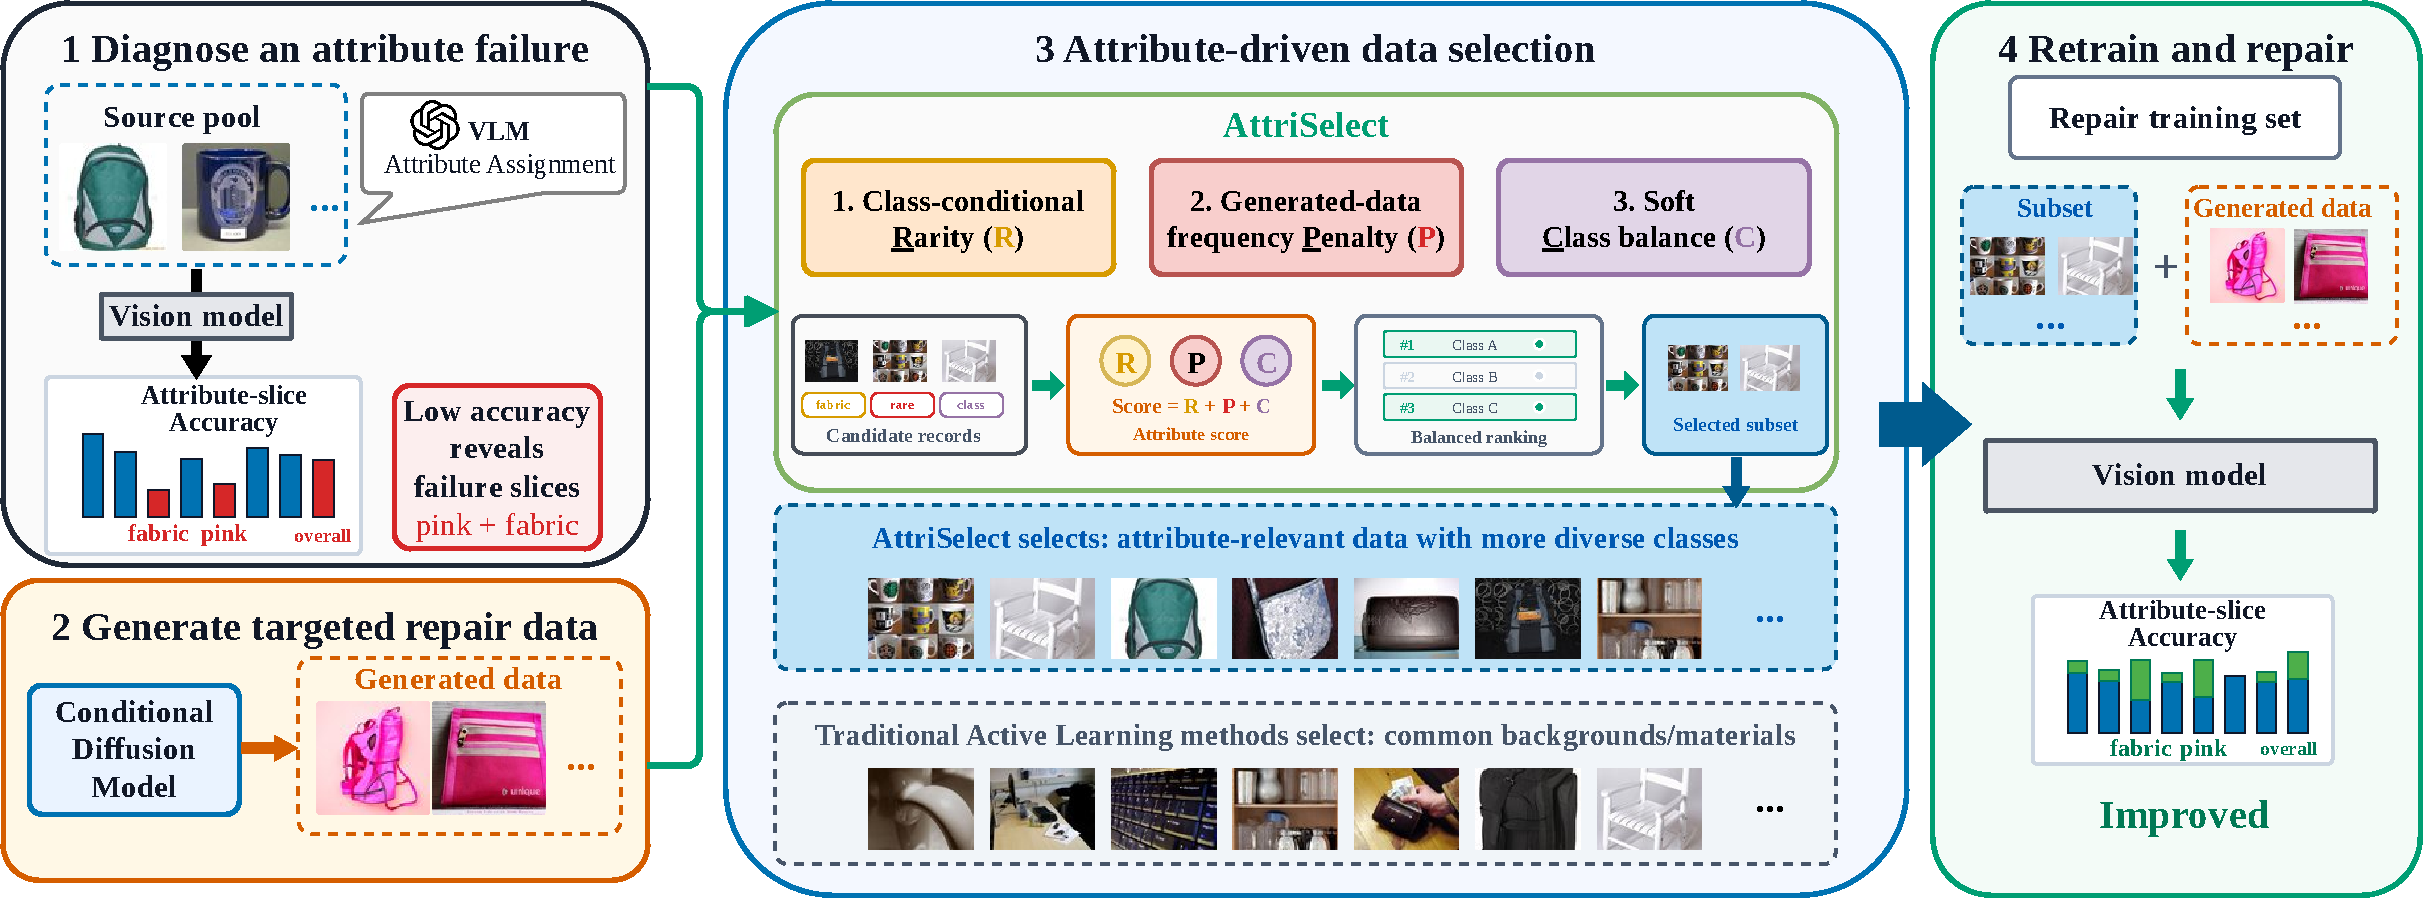
\includegraphics[width=\linewidth]{figures/show/11attriselect_framework.pdf}
\caption{\model framework. Given a diagnosed failure slice and generated images, \model scores source examples with class-conditional rarity, generated-data frequency penalty, and soft class balance, then returns an attribute-driven subset for retraining with the generated repair set.}
\label{fig:attriselect-framework}
\end{figure}

\model is designed as the selection step inside an existing targeted repair pipeline. Figure~\ref{fig:attriselect-framework} summarizes this workflow. The upstream workflow can follow prior model-repair systems such as HiBug and SafeFix~\citep{chen2023hibug,xu2025safefix}. In the experiments reported here, the task-level attribute set $\attrs$ is fixed before selection, and Qwen3-VL~\citep{bai2025qwen3vl} assigns an attribute value $v_{i,a}$ to each training or validation image. Appendix~\ref{app:attribute-assignment-details} gives the task-specific attribute vocabularies and assignment protocol. Using the SafeFix-style ImageNet10 classification setting as a running example, a ResNet-18 classifier~\citep{he2016deep} is then trained to a checkpoint $\theta_t$, after which the repair pipeline analyzes the validation behavior of $f_{\theta_t}$. An attribute slice $T_{\mathrm{bug}}$ is marked as a rare failure case if it is underrepresented in training and underperforms on validation:
\begin{equation}
\label{eq:rare-failure-slice}
|T_{\mathrm{bug}}\cap\dataset_{\mathrm{train}}| < \rho |\dataset_{\mathrm{train}}|,
\qquad
\mathrm{Acc}(T_{\mathrm{bug}}) < \mathrm{Acc}(\dataset_{\mathrm{val}}),
\end{equation}
where $\rho$ is a user-specified rarity threshold. For example, the ImageNet10 pipeline may diagnose a slice whose attribute is \emph{texture} and whose value is \emph{fabric}. A conditional diffusion model, such as ControlNet~\citep{zhang2023adding}, then generates repair images of objects with fabric texture while preserving the class label and other attributes.

\model starts after this upstream diagnosis and generation stage. It takes as input the diagnosed slice, the original source pool with VLM-assigned attributes, and the generated repair images for that slice. The output is a compact source subset $\dataset_{\mathrm{sel}}^{\mathrm{src}}$, which is combined with the generated images and used to continue training or fine-tune the checkpoint $\theta_t$. Thus \model does not replace VLM-based attribute proposal, failure-slice discovery, or conditional image generation. It decides which original training examples should accompany the generated repair data so that retraining preserves source coverage while allocating more budget to real examples that complement the diagnosed repair slice.

\subsection{Attribute-Driven Active Learning}

Given $\dataset_{\mathrm{src}}$ and $\dataset_{\mathrm{gen}}$ for a discovered slice, the goal is to choose a small source subset that still supports the repair. Active learning is a natural tool for this problem: entropy-based uncertainty sampling selects examples with high predictive entropy~\citep{settles2009active}, while CoreSet~\citep{sener2018active}, BADGE~\citep{ash2020deep}, PPAL~\citep{yang2024ppal}, and Uncertainty Herding~\citep{bae2025uncertainty} add coverage, gradient diversity, or detector-side difficulty signals.

For targeted repair, however, the subset must answer a semantic question: which real images best complement the generated examples for the diagnosed failure slice? A subset may provide good coverage of the source distribution in terms of class labels or feature space while still containing very few examples from the rare failure slice itself. Likewise, entropy-based sampling can miss the slice entirely if the model assigns higher uncertainty to unrelated images. Proposition~\ref{prop:al-target-alignment} formalizes this base-rate mismatch.

A second challenge arises because generated repair images alter the attribute distribution seen during retraining. If the generated pool already contains many examples with a target attribute, the source selector should not continue allocating most of its remaining budget to redundant examples of the same attribute. For instance, if generated repair images already emphasize rainy weather, a purely attribute-greedy selector may over-select common rainy street scenes while failing to retain rainy examples from underrepresented classes, unusual viewpoints, or occluded settings. As a result, the repair process can become biased toward the easiest contexts in which the target attribute appears.

\model uses a three-part scoring function to avoid these failure modes. First, the \textbf{class-conditional rarity} term prioritizes attribute values that are rare within their class and therefore more likely to be repair-relevant. Second, the \textbf{generated-data frequency penalty} downweights attribute values that are already well represented by the generated repair images, reducing redundancy between synthetic and source data. Third, the \textbf{soft class-balance} term encourages coverage across classes by increasing the priority of classes that have received insufficient source budget. Together, these components steer selection toward repair-relevant attributes while preventing the subset from collapsing onto repeated synthetic attributes or a small number of easy classes.

\noindent\textbf{Class-conditional rarity.} For a source image $x_i$ with class label $y_i$, let $v_{i,a}$ be the value of attribute $a$ on that image. The rarity term gives higher weight to attribute values that occur fewer times within the same class:
\begin{equation}
\label{eq:rarity-term}
\textcolor{colorR}{R_{i,a}} = \left(\frac{1}{n_a(v_{i,a}\mid y_i)+\varepsilon}\right)^{\alpha}
\end{equation}
where $n_a(v_{i,a}\mid y_i)$ is the number of source examples in class $y_i$ whose attribute $a$ takes value $v_{i,a}$, $\varepsilon > 0$ is a numerical stability constant, and $\alpha \geq 0$ controls how strongly the selector prefers rare attribute values.

This term remains important even after adding generated repair images. Although generated images can make a target attribute less rare in the combined repair pool, they do not make real source examples with that attribute redundant, since the two data sources may differ in image statistics, contextual diversity, learned representations, and other unannotated visual factors. Because repair problems often originate from rare-case failures, class-conditional rarity helps retain real source examples containing rare repair-relevant attributes in the candidate ranking. The role of the generated-data frequency penalty is complementary: rather than promoting rarity, it prevents this preference from repeatedly selecting attribute values that are already heavily represented in the generated repair data.

\noindent\textbf{Generated-data frequency penalty.} Rarity alone can over-select attribute values that are already well covered by the generated repair pool. In the rainy-weather example above, if the generated data already contains many rainy images, the selector should not spend most of its remaining source budget on additional easy rainy cases from similar contexts. Instead, it should retain useful real-source rainy examples while still leaving room for complementary classes, viewpoints, and occlusion patterns. To capture this trade-off, we measure how common each attribute value becomes after combining source and generated data as $\hat{n}_a(v) = n_a^{\mathrm{src}}(v) + \tilde{n}_a^{\mathrm{gen}}(v)$, where $n_a^{\mathrm{src}}(v)$ denotes the source count and $\tilde{n}_a^{\mathrm{gen}}(v)$ denotes the generated count used by the selector after any scaling of the generated pool. Attribute values with larger effective counts receive lower scores:
\begin{equation}
\label{eq:frequency-penalty}
\textcolor{colorP}{P_{i,a}} = -\lambda \cdot \frac{\hat{n}_a(v_{i,a})}{\sum_{v \in \vals_a} \hat{n}_a(v)}
\end{equation}
where $\lambda \geq 0$ controls how strongly the selector penalizes already over-represented attribute values.

We then define the \textbf{base source score} $\bar{s}_i$ by summing the rarity and generated-data frequency terms over the repair attributes:
\begin{equation} \label{eq:base-attribute-score} \bar{s}_i = \sum_{a \in \attrs} \Big( \textcolor{colorR}{R_{i,a}} + \textcolor{colorP}{P_{i,a}} \Big). \end{equation}

Each component addresses a different failure mode in repair-time selection. Setting $\alpha=0$ removes the preference for rare semantic configurations within a class, reducing the selector to a frequency-driven policy. Setting $\lambda=0$ removes the redundancy penalty, allowing the selected subset to repeatedly choose attribute values already well represented in $\dataset_{\mathrm{gen}}$. Without class-aware re-ranking, high-scoring examples may further concentrate within a small subset of classes. As a result, the score is not intended to produce a neutral representative subset; instead, it explicitly allocates source budget toward semantic coverage that is most useful for the diagnosed repair problem.

\noindent\textbf{Soft class balance.} Attribute scores are computed per image, so they can still over-select classes that happen to contain many high-scoring attributes. For example, in a fabric-texture repair, many high-scoring images may come from classes where fabric is visually common, while guitar images may contain the texture only in straps or carrying cases. We correct this with a soft class-balance term. Let $n_{\text{select}}$ be the source-data budget and let $N_{\text{cls}}$ be the number of classes, so the per-class target is $t = n_{\text{select}} / N_{\text{cls}}$. During greedy selection step $k$, a candidate from class $c$ receives the adjusted score
\begin{equation}
\label{eq:class-balance-score}
\tilde{s}_i^{(k)} = \bar{s}_i + \textcolor{colorC}{C_c^{(k)}}, \qquad
\textcolor{colorC}{C_c^{(k)}} = w \cdot \frac{t - n_c^{(k)}}{t},
\end{equation}
where $n_c^{(k)}$ is the number of already selected source samples from class $c$, and $w \geq 0$ controls the strength of soft class balancing. Classes below their target allocation receive a positive correction, while classes above their target receive a negative one. As $w$ increases, the selector behaves more like stratified sampling, with the limiting case $w=\infty$ corresponding to round-robin class quotas. This mechanism preserves the attribute-based ranking from Eq.~\ref{eq:base-attribute-score} within each class while preventing a small subset of classes from dominating the repair set.

Selection is performed greedily. We first compute the base score $\bar{s}_i$ for every source candidate and initialize both the selected set and the per-class counts to zero. At each iteration, every remaining candidate receives the adjusted score $\tilde{s}_i^{(k)}$ from Eq.~\ref{eq:class-balance-score}. The highest-scoring candidate is then added to $\dataset_{\mathrm{sel}}^{\mathrm{src}}$, its class count is updated, and the soft class-balance corrections are recomputed. The process repeats until $n_{\text{select}}$ source examples have been selected. The generated repair set remains fixed throughout this procedure and influences selection only through the frequency counts in Eq.~\ref{eq:frequency-penalty}. As a result, all methods are evaluated under the same generated-data budget. Appendix~\ref{app:attriselect-algorithm} gives the full pseudocode, and Appendix~\ref{app:hyperparameter-details} reports the score hyperparameters used in the experiments.

\subsection{Theoretical Analysis}
\label{subsec:slice-enrichment}

Useful repair subsets should contain rare, underperforming semantic configurations that complement the generated data. Let $N=|\dataset_{\mathrm{src}}|$ be the source-pool size and $m=\lfloor rN\rfloor$ be the budget for $0<r<1$. Let $T\subseteq\dataset_{\mathrm{src}}$ denote the target failure slice, and write $T_c=T\cap\{x_i:y_i=c\}$ and $N_c=|\{x_i:y_i=c\}|$ for class-conditional support.

\begin{tcolorbox}[
    colback=blue!2!white,
    colframe=blue!20!white,
    arc=3pt,
    boxrule=1pt,
    drop shadow,
    breakable
]
\begin{proposition}[Attribute-agnostic AL requires target alignment]
\label{prop:al-target-alignment}
Consider any AL selector that, within class $c$, chooses $B_c$ source examples using only non-attribute information $h_i$, such as uncertainty, logits, embeddings, losses, detector difficulty, coverage, or image distances, and does not use the attribute values $\{v_{i,a}:a\in\attrs\}$. Let $\dataset_{\mathrm{AL}}$ denote its selected source subset. If the target-slice indicator $\mathbf{1}[x_i\in T_c]$ is conditionally independent of $h_i$ given class $c$, with ties and internal randomness independent of the target indicator, then
\begin{equation}
\label{eq:al-target-expectation}
\mathbb{E}\big[|\dataset_{\mathrm{AL}}\cap T_c|\big]
=
B_c\frac{|T_c|}{N_c}.
\end{equation}
Thus an attribute-agnostic AL method can enrich the target slice only when its non-attribute signal is additionally aligned with that slice.
\end{proposition}
\end{tcolorbox}

The expectation in Eq.~\ref{eq:al-target-expectation} reflects a base-rate limit: if a slice is only $2\%$ of class $c$, selecting $100$ class-$c$ examples yields only $2$ target examples in expectation. \model avoids relying on such indirect alignment by observing the attributes that define the diagnosed slice and prioritizing rare repair-relevant values directly. The generated-data penalty and soft class-balance term keep this preference from repeatedly selecting synthetic-like attributes or collapsing onto a few classes. Coverage-based selectors face a similar issue: if target examples form a compact feature region, one or two representatives may cover that region geometrically, even though repair may need more examples from it.

The proposition is stated at the level of selector information rather than for a specific baseline. Stronger baselines such as PPAL and Uncertainty Herding still depend on uncertainty, difficulty, or coverage being aligned with the discovered attribute slice; when this alignment is weak, allocation to the target slice remains proportional to slice prevalence.

\begin{tcolorbox}[
    colback=gray!3!white, 
    colframe=gray!15!white, 
    arc=2pt, 
    boxrule=0.5pt, 
    top=4pt, bottom=4pt, left=6pt, right=6pt
]
\small\noindent See Appendix~\ref{app:theory-analysis} for the \textbf{complete proof}, a coverage-based instance, and score-level conditions under which \model prioritizes rare target-slice examples while limiting class imbalance.
\end{tcolorbox}

\section{Experiments}

\paragraph{Datasets and Tasks}
We evaluate \model on three vision tasks: image classification, pose estimation, and object detection. In all settings, the goal is to test whether attribute-aware source-data selection can choose a subset that improves the model performance and fixes bugs.

For image classification, we follow \safefix~\citep{xu2025safefix}: a ResNet-18 classifier on an ImageNet subset~\citep{deng2009imagenet} with 10 classes, 1,300 images per class, and an 8:1:1 train/validation/test split, denoted ImageNet10. We also evaluate CelebA~\citep{liu2015deep} lipstick-wearing classification with a ResNet-18-based binary classifier and 80,000/10,000/10,000 train/validation/test images. For pose estimation, we follow HiBug2~\citep{chen2025hibug2} on COCO person keypoints~\citep{lin2014microsoft}, using Keypoint R-CNN~\citep{mask-rcnn-2017} with a ResNet-50-FPN backbone~\citep{he2016deep}, 20,000 source training images, and 1,173-image held-out validation and test splits, evaluated by COCO keypoint AP. For object detection, we use KITTI~\citep{geiger2012we} Car and Pedestrian instances converted to YOLO format with 5,000/1,240/1,241 train/validation/test images, and train YOLOv8n. Implementation details are given in Appendix~\ref{app:implementation-details}.

\paragraph{Metrics}
Let $M$ denote the task metric: test accuracy for image classification, COCO keypoint AP for pose estimation, and mAP50--95 for object detection. We focus on targeted improvements for failure cases, which are critical for fairness and safety, while also tracking overall task performance. Following prior work~\citep{lai2023improvingpredictionbackwardcompatiblilitynlp,xu2025safefix}, we report the Fix Rate (FR),
\begin{equation}
\mathrm{FR}(\%)=100\cdot\frac{M_{\mathrm{after}}-M_{\mathrm{before}}}{1-M_{\mathrm{before}}},
\end{equation}
where $M_{\mathrm{before}}$ and $M_{\mathrm{after}}$ are the test metrics before and after repair. In the main FR tables, $M_{\mathrm{before}}$ is $0.7173$ for ImageNet10, $0.9057$ for CelebA, $0.5902$ for COCO, and $0.5626$ for KITTI. For accuracy, FR is the percentage of the original error gap that is corrected; for AP and mAP, it is the normalized improvement toward the maximum score, reported in percent.

\paragraph{Baselines}
We compare \model with seven source-selection baselines. \textbf{\textsc{Random}} samples images uniformly at random. \textbf{\textsc{Stratified}} preserves class proportions during sampling~\citep{neyman1934two}. \textbf{\textsc{Entropy}} is the entropy-based uncertainty baseline; it selects examples with the largest predictive entropy or task-specific confidence-entropy proxy~\citep{settles2009active}. \textbf{\textsc{CoreSet}} uses greedy coverage in embedding space~\citep{sener2018active}. \textbf{\textsc{BADGE}} selects gradient-embedding batches that combine uncertainty and diversity~\citep{ash2020deep}. \textbf{\textsc{PPAL}} is a plug-and-play active-learning baseline for object detection~\citep{yang2024ppal}. \textbf{\textsc{UHerding}} denotes Uncertainty Herding, which combines uncertainty with coverage across label budgets~\citep{bae2025uncertainty}.

Since this repair setting uses both VLM-assigned attributes and generated repair images, we include two robustness checks in the appendix: Appendix~\ref{app:vlm-human-audit} audits the attribute metadata and noise sensitivity, and Appendix~\ref{app:image-generation-effect} tests whether the source-selection trend holds under alternative generators.

\subsection{Main Results}

Table~\ref{tab:main-fr} compares \model with generic source-selection baselines using Fix Rate. All main-result entries are averaged over five random seeds. The original task metrics and variance over five seeds are reported in Appendix~\ref{app:main-metric-tables}.

\noindent\textbf{Analysis.} \model gives the best FR in almost all active source-selection settings, excluding the ratio-$1.0$ full-data references where all selectors are identical. The gap is largest at small budgets, where the selected source subset is highly constrained, and it generally remains at larger budgets. KITTI is the only near-exception: PPAL is slightly higher at ratio $0.7$ by $0.05$ FR points, while \model remains best at the other four KITTI ratios.

Subset selection can also outperform the full-data setting, especially on ImageNet10, CelebA, and COCO. This suggests that the full candidate pool contains noisy, redundant, or target-irrelevant samples, and that selection improves the effective training distribution. In this sense, \model is not only a way to save data or training cost; it also improves data quality and target-slice alignment during repair. The qualitative t-SNE visualizations in Appendix~\ref{app:selection-tsne} further support this interpretation. \model does not simply trace the same regions as generic AL baselines; it selects repair-attribute-related source examples while spreading them across varied visual contexts, consistent with the rarity and soft-balance terms in the score.

KITTI behaves differently at the smallest source budget. At ratio $0.1$, all methods have negative FR. A likely reason is that KITTI has only $5{,}000$ training images, so the selected source subset contains just $500$ real images, unlike ImageNet10, COCO, and CelebA where the same ratio still leaves thousands to tens of thousands of source examples. This negative value should therefore be read as a low-data failure mode: for small detection datasets, an overly small repair subset may not retain enough background, viewpoint, and object-scale variation to improve over the original detector. Under the same generated repair set and source budget, however, \model remains the least damaging option and has the highest FR in this row, indicating the strongest relative source subset under the constrained comparison.

\begin{table}[t]
\centering
\caption{Main repair results across tasks, averaged over five random seeds. Metric: FR (\%).}
\label{tab:main-fr}
\footnotesize
\setlength{\tabcolsep}{1.5pt}
\renewcommand{\arraystretch}{1.2}
\begin{tabular}{l c c c c c c c c >{\columncolor{myblue!8}}c}
\toprule
\rowcolor{sectiongray} \textbf{Dataset} & Ratio & Random & Stratified & Entropy & CoreSet & BADGE & UHerding & PPAL & \cellcolor{myblue!8}\textbf{Ours} \\
\midrule
\multirow{6}{*}{ImageNet10}
& 0.1 & 3.40 & 3.47 & 2.87 & 3.40 & 5.31 & 5.59 & 3.96 & \textbf{6.93} \\
& 0.3 & 4.78 & 6.93 & 4.21 & 6.93 & 8.84 & 10.47 & 7.75 & \textbf{11.28} \\
& 0.5 & 7.32 & 9.66 & 5.59 & 8.03 & 10.47 & 8.38 & 8.84 & \textbf{11.85} \\
& 0.7 & 8.84 & 6.12 & 6.40 & 7.75 & 10.75 & 10.47 & 8.84 & \textbf{12.10} \\
& 0.9 & 10.22 & 10.47 & 10.22 & 6.12 & 9.37 & 11.57 & 11.85 & \textbf{13.76} \\
\noalign{\vskip 1.5pt}\cdashline{3-10}\noalign{\vskip 1.5pt}
& 1.0 & 8.03 & 8.03 & 8.03 & 8.03 & 8.03 & 8.03 & 8.03 & 8.03 \\
\midrule
\multirow{6}{*}{CelebA}
& 0.1 & 4.88 & 2.44 & 7.10 & -6.04 & 3.18 & -1.06 & 5.94 & \textbf{8.48} \\
& 0.3 & 6.04 & 5.30 & 8.70 & 7.95 & 1.91 & 3.50 & 4.03 & \textbf{8.91} \\
& 0.5 & 6.04 & 7.95 & 7.64 & 8.17 & 2.86 & 2.23 & 9.97 & \textbf{13.79} \\
& 0.7 & 2.86 & 8.27 & 10.18 & 6.57 & 8.06 & 5.09 & 6.04 & \textbf{12.09} \\
& 0.9 & 3.18 & 4.56 & 8.27 & 6.04 & 6.04 & 4.56 & 6.57 & \textbf{14.74} \\
\noalign{\vskip 1.5pt}\cdashline{3-10}\noalign{\vskip 1.5pt}
& 1.0 & 6.04 & 6.04 & 6.04 & 6.04 & 6.04 & 6.04 & 6.04 & 6.04 \\
\midrule
\multirow{6}{*}{COCO}
& 0.1 & 3.56 & 5.08 & 5.61 & -0.61 & 2.03 & 2.71 & 1.17 & \textbf{6.86} \\
& 0.3 & 3.37 & 8.32 & 7.64 & 8.64 & 6.12 & 4.32 & 6.42 & \textbf{9.86} \\
& 0.5 & 7.49 & 8.00 & 9.27 & 6.47 & 7.42 & 6.12 & 6.83 & \textbf{10.13} \\
& 0.7 & 6.08 & 9.69 & 9.54 & 9.10 & 8.64 & 6.17 & 7.83 & \textbf{10.18} \\
& 0.9 & 4.61 & 9.49 & 6.54 & 7.32 & 7.59 & 7.05 & 9.74 & \textbf{11.05} \\
\noalign{\vskip 1.5pt}\cdashline{3-10}\noalign{\vskip 1.5pt}
& 1.0 & 8.71 & 8.71 & 8.71 & 8.71 & 8.71 & 8.71 & 8.71 & 8.71 \\
\midrule
\multirow{6}{*}{KITTI}
& 0.1 & -9.65 & -7.27 & -7.52 & -8.89 & -6.95 & -9.24 & -8.32 & \textbf{-5.81} \\
& 0.3 & -0.48 & -1.23 & 0.23 & -0.32 & -0.05 & -1.21 & -1.33 & \textbf{0.46} \\
& 0.5 & 2.13 & 1.23 & 3.20 & 3.04 & 2.29 & 1.12 & 2.17 & \textbf{3.36} \\
& 0.7 & 3.20 & 3.06 & 3.34 & 3.34 & 2.08 & 3.25 & \textbf{3.57} & 3.52 \\
& 0.9 & 4.37 & 4.66 & 4.66 & 3.54 & 4.21 & 4.85 & 3.89 & \textbf{5.12} \\
\noalign{\vskip 1.5pt}\cdashline{3-10}\noalign{\vskip 1.5pt}
& 1.0 & 5.30 & 5.30 & 5.30 & 5.30 & 5.30 & 5.30 & 5.30 & 5.30 \\
\bottomrule
\end{tabular}
\end{table}

\subsection{Computational Efficiency}

\model is also cheaper than generic active-learning selectors. Its
selection cost is dominated by counting VLM-assigned attribute values and
sorting candidates, while uncertainty, coverage, and gradient-embedding
baselines require model scoring, embedding comparisons, or iterative diversity
updates. Table~\ref{tab:selection-efficiency} reports source-subset selection
time on COCO and CelebA for the three ratios used in the main small-to-medium
budget comparison. The source pools contain 20,000 COCO training images and
80,000 CelebA training images. Random and stratified sampling have negligible
algorithmic selection cost after excluding data loading and export overhead;
we keep them in the table as zero-cost references.

\begin{table}[t]
\centering
\caption{Source-subset selection time. Units are seconds (s), minutes (m), and hours (h). Speedup is measured against the fastest non-attribute active-learning baseline in the same row.}
\label{tab:selection-efficiency}
\footnotesize
\setlength{\tabcolsep}{1.2pt}
\renewcommand{\arraystretch}{1.2}
\begin{tabular}{l c c c c c c c c >{\columncolor{myblue!8}}c}
\toprule
\rowcolor{sectiongray} Dataset & Ratio & Random & Stratified & Entropy & CoreSet & BADGE & UHerding & PPAL & \cellcolor{myblue!8}\textbf{Ours / speedup} \\
\midrule
COCO & 0.1 & 0s & 0s & 863s & 5m & 21m & 86s & 67s & \textbf{0.29s / 231$\times$} \\
COCO & 0.3 & 0s & 0s & 865s & 15m & 1h & 93s & 85s & \textbf{0.30s / 283$\times$} \\
COCO & 0.5 & 0s & 0s & 865s & 25m & 2h & 94s & 90s & \textbf{0.32s / 281$\times$} \\
\midrule
CelebA & 0.1 & 0s & 0s & 49s & 45m & 2h & 63s & 46s & \textbf{0.42s / 110$\times$} \\
CelebA & 0.3 & 0s & 0s & 51s & 3h & 5h & 65s & 51s & \textbf{0.51s / 100$\times$} \\
CelebA & 0.5 & 0s & 0s & 54s & 5h & 9h & 61s & 61s & \textbf{1.37s / 39$\times$} \\
\bottomrule
\end{tabular}
\end{table}

\model selects each subset in less than two seconds. The fastest non-attribute
active-learning baseline takes tens of seconds, and coverage or
gradient-embedding methods can take minutes to hours. Even against the fastest
nontrivial baseline in each row, \model is at least $39\times$ faster on
CelebA and more than $230\times$ faster on COCO.

\subsection{Attribute-Slice Accuracy Differences}

For each attribute slice, we report the accuracy difference
$M_{\mathrm{after}}-M_{\mathrm{before}}$, where $M_{\mathrm{before}}$ is
measured at the original vision model checkpoint $\theta_t$ and
$M_{\mathrm{after}}$ is measured after retraining. For ImageNet10
classification, $M$ is accuracy. Positive values therefore indicate
slice-level improvement after repair. Figure~\ref{fig:imagenet-ratio05-attribute-delta} reports these differences for ImageNet10 at source ratio $0.5$.

\begin{figure}[t]
\centering
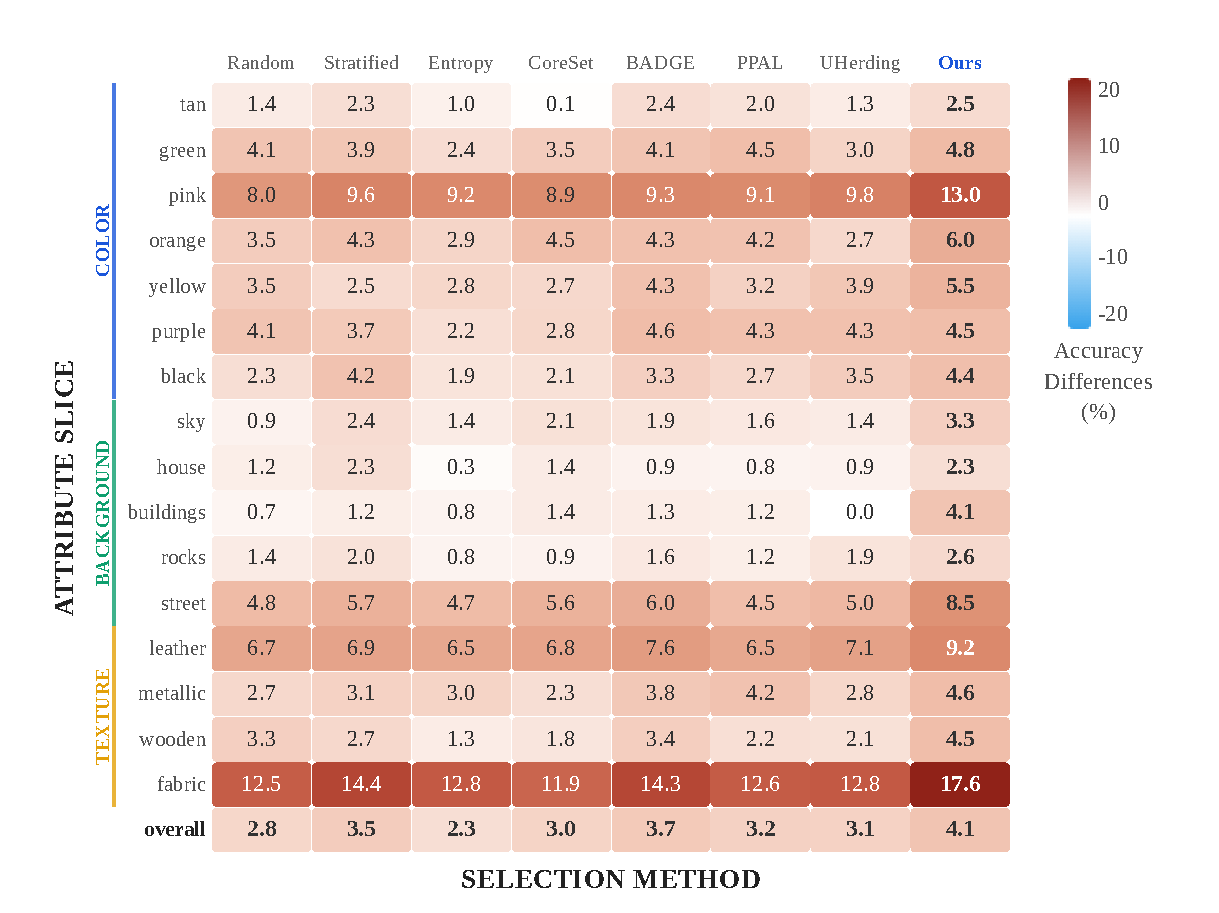
\includegraphics[width=0.86\linewidth,trim={0 9pt 0 26pt},clip]{figures/show/heatmap_.pdf}
\caption{ImageNet10 ratio-$0.5$ attribute-slice accuracy differences. \model gives larger gains on the targeted attribute families, with the strongest gains on the exact repair values.}
\label{fig:imagenet-ratio05-attribute-delta}
\end{figure}

All methods use the same generated repair images and differ only in the
selected source subset. The generated data targets pink color and fabric
texture. \model gives the largest gains on the targeted attribute families,
especially the exact repair values pink and fabric, indicating that the
selected source subset improves target-slice alignment rather than only
changing overall accuracy. A COCO pose-estimation version with the full
annotated attribute vocabulary is provided in
Appendix~\ref{app:attribute-slice-heatmaps}.

\subsection{Failure-Slice Repair Counts}

\begin{wraptable}{r}{0.27\linewidth}
\vspace{-1.0em}
\centering
\caption{COCO repaired slices out of 12.}
\label{tab:coco-bug-repair-counts}
\scriptsize
\setlength{\tabcolsep}{3pt}
\renewcommand{\arraystretch}{0.9}
\begin{tabular}{c c >{\columncolor{myblue!8}}c}
\toprule
Ratio & Best AL & Ours \\
\midrule
0.1 & 7 & \textbf{10} \\
0.3 & 8 & \textbf{10} \\
0.5 & 10 & \textbf{11} \\
0.7 & 10 & \textbf{11} \\
0.9 & 10 & \textbf{11} \\
\bottomrule
\end{tabular}
\vspace{-1.2em}
\end{wraptable}

We also evaluate repair at the level of discovered failure slices. In the
upstream bug-discovery stage for COCO, 12 failure slices are identified. With
the proposed framework, \model repairs 10 of these slices already at source
ratio $0.1$, whereas the strongest active-learning baseline repairs 7 slices
at the same ratio. The strongest baseline reaches 10 repaired slices only from
source ratio $0.5$ onward, while \model repairs 11 slices at ratios $0.5$,
$0.7$, and $0.9$.

\subsection{Ablation Study}

We ablate the three score components on ImageNet10 classification repair to test whether the gains come from a single term or from their combination. Table~\ref{tab:imagenet-rpc-ablation} reports test accuracy for all component subsets. The full $\textcolor{colorR}{R}+\textcolor{colorP}{P}+\textcolor{colorC}{C}$ setting combines rarity $\textcolor{colorR}{R}$, generated-data frequency penalty $\textcolor{colorP}{P}$, and soft class balance $\textcolor{colorC}{C}$. The full $\textcolor{colorR}{R}+\textcolor{colorP}{P}+\textcolor{colorC}{C}$ setting is the most stable choice in this ablation, giving the best result at every ratio. The leave-one-component-out drops from the full setting are nearly identical: removing $\textcolor{colorR}{R}$ drops test accuracy by $0.00942$ on average, removing $\textcolor{colorP}{P}$ by $0.00940$, and removing $\textcolor{colorC}{C}$ by $0.00940$. Thus the ablation supports a complementarity claim rather than a single dominant-component claim on ImageNet10. Single-component variants are weaker on average ($\textcolor{colorR}{R}$: $0.74198$, $\textcolor{colorP}{P}$: $0.74038$, $\textcolor{colorC}{C}$: $0.73814$) than the full setting ($0.74892$), showing that each component alone is insufficient. A COCO pose-estimation component ablation with a broadly similar trend is reported in Appendix~\ref{app:coco-rpc-ablation}.

\begin{table}[t]
\centering
\caption{ImageNet10 classification attribute-score component ablation. Metric: test accuracy.}
\label{tab:imagenet-rpc-ablation}
\footnotesize
\setlength{\tabcolsep}{4pt}
\begin{tabular}{c c c c c c c c >{\columncolor{myblue!8}}c}
\toprule
Ratio & none & $\textcolor{colorR}{R}$ & $\textcolor{colorP}{P}$ & $\textcolor{colorC}{C}$ & $\textcolor{colorP}{P}+\textcolor{colorC}{C}$ & $\textcolor{colorR}{R}+\textcolor{colorC}{C}$ & $\textcolor{colorR}{R}+\textcolor{colorP}{P}$ & \cellcolor{myblue!8}$\textcolor{colorR}{\boldsymbol{R}}+\textcolor{colorP}{\boldsymbol{P}}+\textcolor{colorC}{\boldsymbol{C}}$ \\
\midrule
0.1 & 0.7269 & 0.7300 & 0.7262 & 0.7277 & 0.7359 & 0.7308 & 0.7315 & \textbf{0.7369} \\
0.3 & 0.7308 & 0.7415 & 0.7392 & 0.7392 & 0.7308 & 0.7369 & 0.7315 & \textbf{0.7492} \\
0.5 & 0.7400 & 0.7415 & 0.7408 & 0.7346 & 0.7369 & 0.7415 & 0.7446 & \textbf{0.7508} \\
0.7 & 0.7423 & 0.7469 & 0.7431 & 0.7415 & 0.7431 & 0.7469 & 0.7477 & \textbf{0.7515} \\
0.9 & 0.7462 & 0.7500 & 0.7526 & 0.7477 & 0.7508 & 0.7415 & 0.7423 & \textbf{0.7562} \\
\bottomrule
\end{tabular}
\end{table}
% We conduct experiments on ImageNet-10 (multi-class) and CelebA (binary, targeting the `redhair\_brownskin' subgroup correlation). We employ a standard ResNet-18 architecture, initiating with pretrained weights and utilizing the AdamW optimizer. 

% \subsection{\model vs. Long-Tail Learning Baselines}

% We isolate the effect of \model against four standard LTL algorithms: Focal Loss \citep{lin2017focal}, Class-Balanced Loss, Oversampling (via WeightedRandomSampler), and LDAM Loss \citep{cao2019learning}. To ensure a fair comparison, the LTL baselines were trained exclusively on the original datasets without access to the targeted synthetic augmentation provided by \model.

% \begin{table}[h]
% \caption{Performance comparison of \model vs. LTL baselines on ResNet-18. \model leverages synthetic subgroups, effectively rescuing bugs where standard reweighting methods fail.}
% \centering
% \begin{tabular}{l cc cc}
% \toprule
% \textbf{Method} & \textbf{CelebA Test ACC} & \textbf{Fix Bugs} & \textbf{ImageNet Test ACC} & \textbf{Fix Bugs} \\
% \midrule
% Base Model & 90.57\% & - & 71.73\% & - \\
% Focal Loss & 91.40\% & 8/13 & 68.80\% & 11/17 \\
% Class-Balanced Loss & 91.20\% & 8/13 & 72.70\% & 13/17 \\
% Oversampling & 91.00\% & 8/13 & 72.90\% & 14/17 \\
% LDAM & 91.40\% & 8/13 & 71.20\% & 12/17 \\
% \midrule
% \textbf{/model (Ours)} & \textbf{91.92\%} & - & \textbf{74.88\%} & - \\
% \bottomrule
% \end{tabular}
% \end{table}

% The results demonstrate that while algorithmic reweighting techniques provide marginal improvements over the base model, they are fundamentally insufficient for repairing unannotated, intersectional attribute failures compared to SafeFix's target-augmented methodology.

% \subsection{Active Learning Strategy Ablations}

% To validate the efficiency of our Attribute-Driven strategy in curating augmented datasets, we compare it against standard Active Learning regimes across various integration sub-ratios ($0.1$ through $0.9$). The models were trained learning rate of $1e-5$ for 15 epochs. 

% \begin{table}[h]
% \caption{Comparison of Top-Performing Selection Strategies on ImageNet (ResNet-18) at various subset sampling ratios. Our Attribute strategy utilizes generated captions from LLMs (BLIP, Qwen3, InternVL3).}
% \centering
% \resizebox{\columnwidth}{!}{
% \begin{tabular}{l ccc c}
% \toprule
% \textbf{Strategy} & \textbf{Ratio=0.1} Test/Val & \textbf{Ratio=0.3} Test/Val & \textbf{Ratio=0.5} Test/Val & \textbf{Ratio=0.9} Test/Val \\
% \midrule
% Random & 0.7269 / 0.7069 & 0.7308 / 0.7208 & 0.7400 / 0.7162 & 0.7482 / 0.7154 \\
% Stratified & 0.7271 / 0.7154 & 0.7369 / 0.7162 & 0.7446 / 0.7200 & 0.7469 / 0.7146 \\
% Coreset & 0.7269 / 0.7115 & 0.7369 / 0.7162 & 0.7400 / 0.7185 & 0.7346 / 0.7169 \\
% Uncertainty Stratified & 0.7254 / 0.7185 & 0.7292 / 0.7131 & 0.7331 / 0.7146 & 0.7462 / 0.7100 \\
% Hierarchical & 0.7269 / 0.7115 & 0.7346 / 0.7092 & 0.7385 / 0.7138 & 0.7362 / 0.7177 \\
% \midrule
% Attribute (BLIP) & 0.7277 / 0.7200 & 0.7369 / 0.7185 & 0.7408 / 0.7131 & 0.7400 / 0.7177 \\
% Attribute (Qwen3) & 0.7331 / 0.7231 & 0.7354 / 0.7077 & 0.7362 / 0.7138 & 0.7492 / 0.7108 \\
% \textbf{Attribute (InternVL3)} & \textbf{0.7346} & \textbf{0.7385} & \textbf{0.7495} & \textbf{0.7531} \\
% \bottomrule
% \end{tabular}
% }
% \end{table}

% The Attribute-Driven strategy continuously outperforms traditional geometry-based (Coreset) and balanced (Stratified) methodologies at almost every data budget. Further utilizing advanced Vision-Language Models like InternVL3 to source the attribute metadata yields compounding performance benefits.


% \subsection{Parameter Scaling Analysis}

% By adjusting the weights of $R$, $P$, and $C$, we explored the behavioral boundaries of our strategy (sub-ratio $0.3$). 

% \begin{itemize}
%     \item \textbf{Pure Greedy ($R=1.0, P=10.0, C=0.0$)}: Test ACC 0.7215. Without class-level Stratification quotas, throwing out all logic except Frequency Penalty and Rarity leads to performance drops in fine-tuning, emphasizing the value of our soft $C$ score.
%     \item \textbf{Aggressive Exploration ($R=0.8, P=10.0, C=4.0$)}: Test ACC \textbf{0.7415}. By loosening the absolute restriction on stratification and vastly scaling up Rarity tracking, the model dynamically locates critical edge cases. The extreme Frequency Penalty ($P=10$) adequately prevents the network from collapsing entirely onto the synthetic injection vectors.
% \end{itemize}

\section{Conclusion}

We studied targeted vision model repair as a repair-time source-selection problem. In this setting, a failure slice has been diagnosed and targeted repair images have been generated; the remaining question is which source examples should accompany those generated images during retraining. \model addresses this question with an attribute-driven score that combines class-conditional rarity, generated-data frequency control, and soft class balancing. The analysis shows when this score enriches rare target slices relative to attribute-agnostic selectors, and the experiments across classification, pose estimation, and detection indicate that structured attribute metadata provides a useful signal beyond uncertainty, coverage, and gradient-embedding scores. \model is therefore best viewed as one component in a localized repair pipeline, not as a replacement for upstream bug discovery or image generation.

\subsection*{Reproducibility statement}
Our methodology, hyperparameter configurations, selection algorithm, and mathematical analysis are described in Section~\ref{sec:method} and expanded in the Appendix. We provide detailed implementation and experimental setups in Appendix~\ref{app:implementation-details}, the complete attribute-driven selection algorithm in Appendix~\ref{app:attriselect-algorithm}, and theoretical proofs in Appendix~\ref{app:theory-analysis}.

\subsection*{Ethics statement}
This work studies data subset selection for vision model repair using established public benchmarks and standard diagnostic pipelines. It does not introduce new human-subject studies or sensitive personally identifiable information. Limitations and broader potential impacts are discussed in Appendix~\ref{app:limitations}.

\bibliography{ref}
\bibliographystyle{iclr2027_conference}

\newpage
\appendix
\begin{center}
    \LARGE \textbf{Appendix}
    \vspace{1em}
\end{center}

\begin{tcolorbox}[
    colback=gray!2!white,
    colframe=gray!20!white,
    arc=4pt,
    boxrule=0.5pt,
    left=12pt, right=12pt, top=10pt, bottom=10pt,
    title=\textbf{Appendix Outline},
    coltitle=black,
    fonttitle=\bfseries\large,
    colbacktitle=gray!10!white,
    rounded corners,
    drop shadow
]
\startcontents[appendix]
\printcontents[appendix]{l}{1}{\setcounter{tocdepth}{2}}
\end{tcolorbox}
\vspace{2.5em}

\section{Glossary}
\label{app:glossary}

The notations are summarized in Table~\ref{tab:glossary}.

\begin{table}[htbp]
\centering
\caption{Glossary of variables and symbols used in this paper.}
\label{tab:glossary}
\small
\begin{tabular}{ll}
\toprule
\rowcolor{sectiongray} \textbf{Symbol} & \textbf{Description} \\
\midrule
$\mathcal{X}$ & Input image space \\
$\mathcal{Y}$ & Label space \\
$\mathcal{D}_{\mathrm{src}}$ & Source training image dataset \\
$\mathcal{D}_{\mathrm{gen}}$ & Generated repair image pool \\
$\mathcal{D}_{\mathrm{repair}}$ & Retraining dataset composed of selected source and generated images \\
$\mathcal{D}_{\mathrm{sel}}^{\mathrm{src}}$ & Selected subset of the source dataset for retraining \\
$\mathcal{D}_{\mathrm{sel}}^{\mathrm{gen}}$ & Generated subset used for repair \\
$\mathcal{A}$ & Task-level attribute vocabulary proposed by the VLM \\
$\mathcal{V}_a$ & Vocabulary of candidate values for attribute $a \in \mathcal{A}$ \\
$v_{i,a}$ & Attribute value assigned to image $x_i$ for attribute $a$ \\
$s_i$ & Final selection score of source candidate $x_i$ \\
$\bar{s}_i$ & Base selection score (rarity score minus frequency penalty) \\
$n_a(v \mid c)$ & Class-conditional count of attribute value $v$ in class $c$ in the source pool \\
$\hat{n}_a(v)$ & Frequency count of attribute value $v$ in the generated repair pool \\
$n_c^{(k)}$ & Number of selected source samples from class $c$ at selection iteration $k$ \\
$\alpha$ & Rarity exponent \\
$\lambda$ & Frequency penalty weight \\
$w$ & Soft class-balancing weight \\
$T$ & Target failure slice diagnosed by the debugging pipeline \\
$T_c$ & Class-conditional target failure slice \\
$B_c$ & Number of selected class-$c$ examples (source budget) \\
$N_c$ & Total support size of class $c$ in the source pool \\
\bottomrule
\end{tabular}
\end{table}


\section{Implementation Details}
\label{app:implementation-details}

\paragraph{Random seeds.}
For the main-result tables, we run each setting with five seeds: 0, 42, 1234, 3407, and 2024. Unless stated otherwise, auxiliary analyses outside the main-result tables use seed 42.

\paragraph{Hardware and datasets.}
All experiments use a GPU cluster with four NVIDIA RTX A5000 GPUs. For image classification, we follow \safefix~\citep{xu2025safefix}: a ResNet-18 classifier~\citep{he2016deep} on an ImageNet subset~\citep{deng2009imagenet} with 10 classes, 1,300 images per class, and an 8:1:1 train/validation/test split, denoted ImageNet10. The ImageNet10 classes are \texttt{backpack}, \texttt{barber chair}, \texttt{coffee mug}, \texttt{desk}, \texttt{electric guitar}, \texttt{park bench}, \texttt{pitcher}, \texttt{purse}, \texttt{rocking chair}, and \texttt{water bottle}. We also evaluate CelebA~\citep{liu2015deep} lipstick-wearing classification with a ResNet-18-based binary classifier and 80,000/10,000/10,000 train/validation/test images. For pose estimation, we follow HiBug2~\citep{chen2025hibug2} on COCO person keypoints~\citep{lin2014microsoft}, using Keypoint R-CNN~\citep{mask-rcnn-2017} with a ResNet-50-FPN backbone~\citep{he2016deep}, 20,000 source training images, and 1,173-image held-out validation and test splits. For object detection, we use KITTI~\citep{geiger2012we} Car and Pedestrian instances converted to YOLO format with 5,000/1,240/1,241 train/validation/test images, and train YOLOv8n.

\paragraph{Training and repair schedule.}
For ImageNet10 classification, the diagnosis-stage ResNet-18 model is trained with cross-entropy loss and Adam~\citep{kingma2015adam}, using learning rate $1\times10^{-4}$, weight decay $1\times10^{-3}$, batch size 64, and 30 epochs. During repair, we train with the selected source subset and the generated repair images for 15 epochs using learning rate $1\times10^{-5}$. For CelebA, COCO, and KITTI, the repair-stage epoch count is set to half of the corresponding diagnosis-stage training schedule, with the same repair-stage learning rate $1\times10^{-5}$.

\paragraph{Image generation.}
For the generated repair images used in the main results, we use \controlnet~\citep{zhang2023adding}, a conditional diffusion model based on Stable Diffusion 1.5~\citep{rombach2022high}. The model is conditioned on soft HED boundaries~\citep{xie2015holistically} extracted from source images and uses 30 DDIM inference steps~\citep{ddim}. The soft boundary condition helps preserve object structure during edits, which is useful for attribute changes such as recoloring, material changes, and weather or style edits.

\paragraph{Attribute proposal and assignment.}
We use vision-language models (VLMs) in two separate roles. First, a VLM proposes the semantic attribute vocabulary $\attrs$ for a task. For example, in KITTI object detection, GPT-5~\citep{openai2025gpt5} is used to define candidate visual attributes such as color, weather, scale, viewpoint, occlusion, truncation, and motion state. Second, a VLM assigns attribute values to source and generated images. In the experiments reported in this paper, we use Qwen3-VL~\citep{bai2025qwen3vl} for this assignment step. For the KITTI object-detection repair, color and weather are the attribute fields tied to the discovered repair slice.

\paragraph{Generation and assignment cost.}
Generating 1,000 images with ControlNet takes slightly over one hour on our cluster. Assigning attributes to these images with Qwen3-VL takes about 10--20 minutes, depending on the queried attribute set.


\section{\modelplain Algorithm}
\label{app:attriselect-algorithm}

\begin{figure}[htbp]
\begin{tcolorbox}[
    colback=white,
    colframe=myblue!75!black,
    colbacktitle=myblue!12!white,
    coltitle=myblue!60!black,
    title=\textbf{Algorithm 1: \model Source Selection for Targeted Repair},
    fonttitle=\bfseries,
    rounded corners,
    drop shadow,
    left=6pt,right=6pt,top=4pt,bottom=4pt,
    width=0.98\linewidth
]
\label{alg:attriselect}
\begin{algorithmic}[1]
\Require Source pool $\dataset_{\mathrm{src}}=\{(x_i,y_i,A_i)\}_{i=1}^{N}$ with VLM-assigned attribute records $A_i=\{v_{i,a}:a\in\attrs\}$; generated repair pool $\dataset_{\mathrm{gen}}$ with attribute records; source-selection budget $n_{\mathrm{select}}$; score parameters $\alpha$, $\lambda$, $w$; numerical constant $\varepsilon$
\Ensure Selected source subset $\dataset_{\mathrm{sel}}^{\mathrm{src}}$
\State Compute class-conditional source counts $n_a(v\mid c)$ for every attribute $a$, value $v$, and class $c$
\State Compute effective attribute counts $\hat{n}_a(v)=n_a^{\mathrm{src}}(v)+\tilde{n}_a^{\mathrm{gen}}(v)$ using the source pool and generated repair pool
\ForAll{$(x_i,y_i,A_i)\in\dataset_{\mathrm{src}}$}
    \State $\textcolor{colorR}{R_{i,a}}\gets \left(n_a(v_{i,a}\mid y_i)+\varepsilon\right)^{-\alpha}$ for each $a\in\attrs$
    \State $\textcolor{colorP}{P_{i,a}}\gets -\lambda\cdot \hat{n}_a(v_{i,a}) \big/ \sum_{v\in\vals_a}\hat{n}_a(v)$ for each $a\in\attrs$
    \State $\bar{s}_i\gets \sum_{a\in\attrs}\left(\textcolor{colorR}{R_{i,a}}+\textcolor{colorP}{P_{i,a}}\right)$
\EndFor
\State $\dataset_{\mathrm{sel}}^{\mathrm{src}}\gets \emptyset$; initialize selected class counts $n_c\gets 0$ for all classes
\State Set the soft per-class target $t\gets n_{\mathrm{select}}/N_{\mathrm{cls}}$
\While{$|\dataset_{\mathrm{sel}}^{\mathrm{src}}|<n_{\mathrm{select}}$}
    \ForAll{remaining candidates $x_i\notin\dataset_{\mathrm{sel}}^{\mathrm{src}}$ with class $y_i=c$}
        \State $\textcolor{colorC}{C_c}\gets w\cdot(t-n_c)/t$
        \State $\tilde{s}_i\gets \bar{s}_i+\textcolor{colorC}{C_c}$
    \EndFor
    \State Select $x_j\gets \arg\max_{x_i\notin\dataset_{\mathrm{sel}}^{\mathrm{src}}}\tilde{s}_i$
    \State $\dataset_{\mathrm{sel}}^{\mathrm{src}}\gets \dataset_{\mathrm{sel}}^{\mathrm{src}}\cup\{x_j\}$; update $n_{y_j}\gets n_{y_j}+1$
\EndWhile
\State \Return $\dataset_{\mathrm{sel}}^{\mathrm{src}}$
\end{algorithmic}
\end{tcolorbox}
\end{figure}

The generated repair pool is fixed during selection. It affects \model only through the effective attribute counts in the frequency-penalty term, so all compared selectors use the same generated-data budget.


\section{Attribute Assignment Details}
\label{app:attribute-assignment-details}

\noindent\textbf{CelebA and ImageNet10.}
Attribute assignments for CelebA use the official CelebA annotations and follow the SafeFix setting~\citep{xu2025safefix}. ImageNet10 does not provide official attribute annotations, so we follow the SafeFix-style ImageNet10 protocol: define task-level attribute fields such as \texttt{color}, \texttt{background}, and \texttt{texture}, then assign closed-set attribute values to each image with the VLM. These assignments are used only as selection metadata for \model and for post-training slice diagnostics; benchmark labels remain the source of the reported task metrics.

\noindent\textbf{COCO and KITTI.}
For COCO pose estimation and KITTI object detection, we follow HiBug2~\citep{chen2025hibug2} and use task-specific closed-set attribute fields proposed before source selection. We take KITTI as a concrete example. GPT-5~\citep{openai2025gpt5} proposes 10 representative object-detection categories, listed in Figure~\ref{tab:kitti-attribute-corpus}. Each category has a predefined set of candidate values, a natural-language prompt template, and a corresponding query directed to Qwen3-VL~\citep{bai2025qwen3vl}. The repair fields used in the main KITTI experiments are color and weather; the remaining fields are retained for broader slice analysis and diagnostics.

\begin{figure}[htbp]
\centering
\caption{KITTI object-detection attribute corpus used for VLM assignment.}
\label{tab:kitti-attribute-corpus}
\begin{tcolorbox}[
    colback=blue!2!white,
    colframe=blue!15!black,
    title=\textbf{KITTI Attribute Corpus \& VLM Prompts},
    fonttitle=\bfseries,
    rounded corners,
    drop shadow,
    left=6pt,
    right=6pt,
    top=4pt,
    bottom=4pt,
    fontupper=\small,
    width=0.98\linewidth
]
\textit{Note: The placeholder \texttt{\#1} is replaced by a candidate value from the corresponding category.}
\vspace{0.8em}

\begin{description}
    \setlength{\itemsep}{0.6em}
    \item[\texttt{color}:] \texttt{white}, \texttt{black}, \texttt{gray}, \texttt{silver}, \texttt{red}, \texttt{blue}, \texttt{green}, \texttt{yellow}, \texttt{brown} \\
    \textcolor{gray}{\textbf{Prompt:}} \texttt{a \#1 main target object in a driving scene}

    \item[\texttt{object\_scale}:] \texttt{small}, \texttt{medium}, \texttt{large} \\
    \textcolor{gray}{\textbf{Prompt:}} \texttt{a \#1 target object in a driving scene}

    \item[\texttt{viewpoint}:] \texttt{front}, \texttt{rear}, \texttt{side}, \texttt{front-side}, \texttt{rear-side} \\
    \textcolor{gray}{\textbf{Prompt:}} \texttt{a \#1 view of the main target object in a driving scene}

    \item[\texttt{occlusion}:] \texttt{none}, \texttt{partial}, \texttt{heavy} \\
    \textcolor{gray}{\textbf{Prompt:}} \texttt{a \#1 occluded target object in a driving scene}

    \item[\texttt{truncation}:] \texttt{none}, \texttt{partial}, \texttt{heavy} \\
    \textcolor{gray}{\textbf{Prompt:}} \texttt{a \#1 truncated target object in a driving scene}

    \item[\texttt{motion\_state}:] \texttt{moving}, \texttt{stationary} \\
    \textcolor{gray}{\textbf{Prompt:}} \texttt{a \#1 target object in a driving scene}

    \item[\texttt{background\_style}:] \texttt{city street}, \texttt{residential street}, \texttt{highway}, \texttt{parking area}, \texttt{service lane}, \texttt{tree-lined road} \\
    \textcolor{gray}{\textbf{Prompt:}} \texttt{a driving scene on a \#1}

    \item[\texttt{traffic\_density}:] \texttt{sparse}, \texttt{light}, \texttt{moderate}, \texttt{heavy} \\
    \textcolor{gray}{\textbf{Prompt:}} \texttt{a driving scene with \#1 traffic}

    \item[\texttt{lighting\_condition}:] \texttt{bright}, \texttt{overcast}, \texttt{strong shadows}, \texttt{glare}, \texttt{dim} \\
    \textcolor{gray}{\textbf{Prompt:}} \texttt{a driving scene with \#1 lighting}

    \item[\texttt{weather}:] \texttt{clear}, \texttt{cloudy}, \texttt{rainy}, \texttt{foggy}, \texttt{snowy} \\
    \textcolor{gray}{\textbf{Prompt:}} \texttt{a driving scene in \#1 weather}
\end{description}
\end{tcolorbox}
\end{figure}


\section{Attribute-Slice Heatmaps}
\label{app:attribute-slice-heatmaps}

Figure~\ref{fig:coco-ratio05-attribute-delta} reports the corresponding
ratio-$0.5$ COCO pose-estimation slice analysis over the full annotated
attribute vocabulary. The targeted repair values are clothes color brown and
rainy weather. As in the ImageNet10 example, the largest gains appear on the
targeted values, while the remaining attributes show smaller changes.

\begin{figure}[p]
\centering
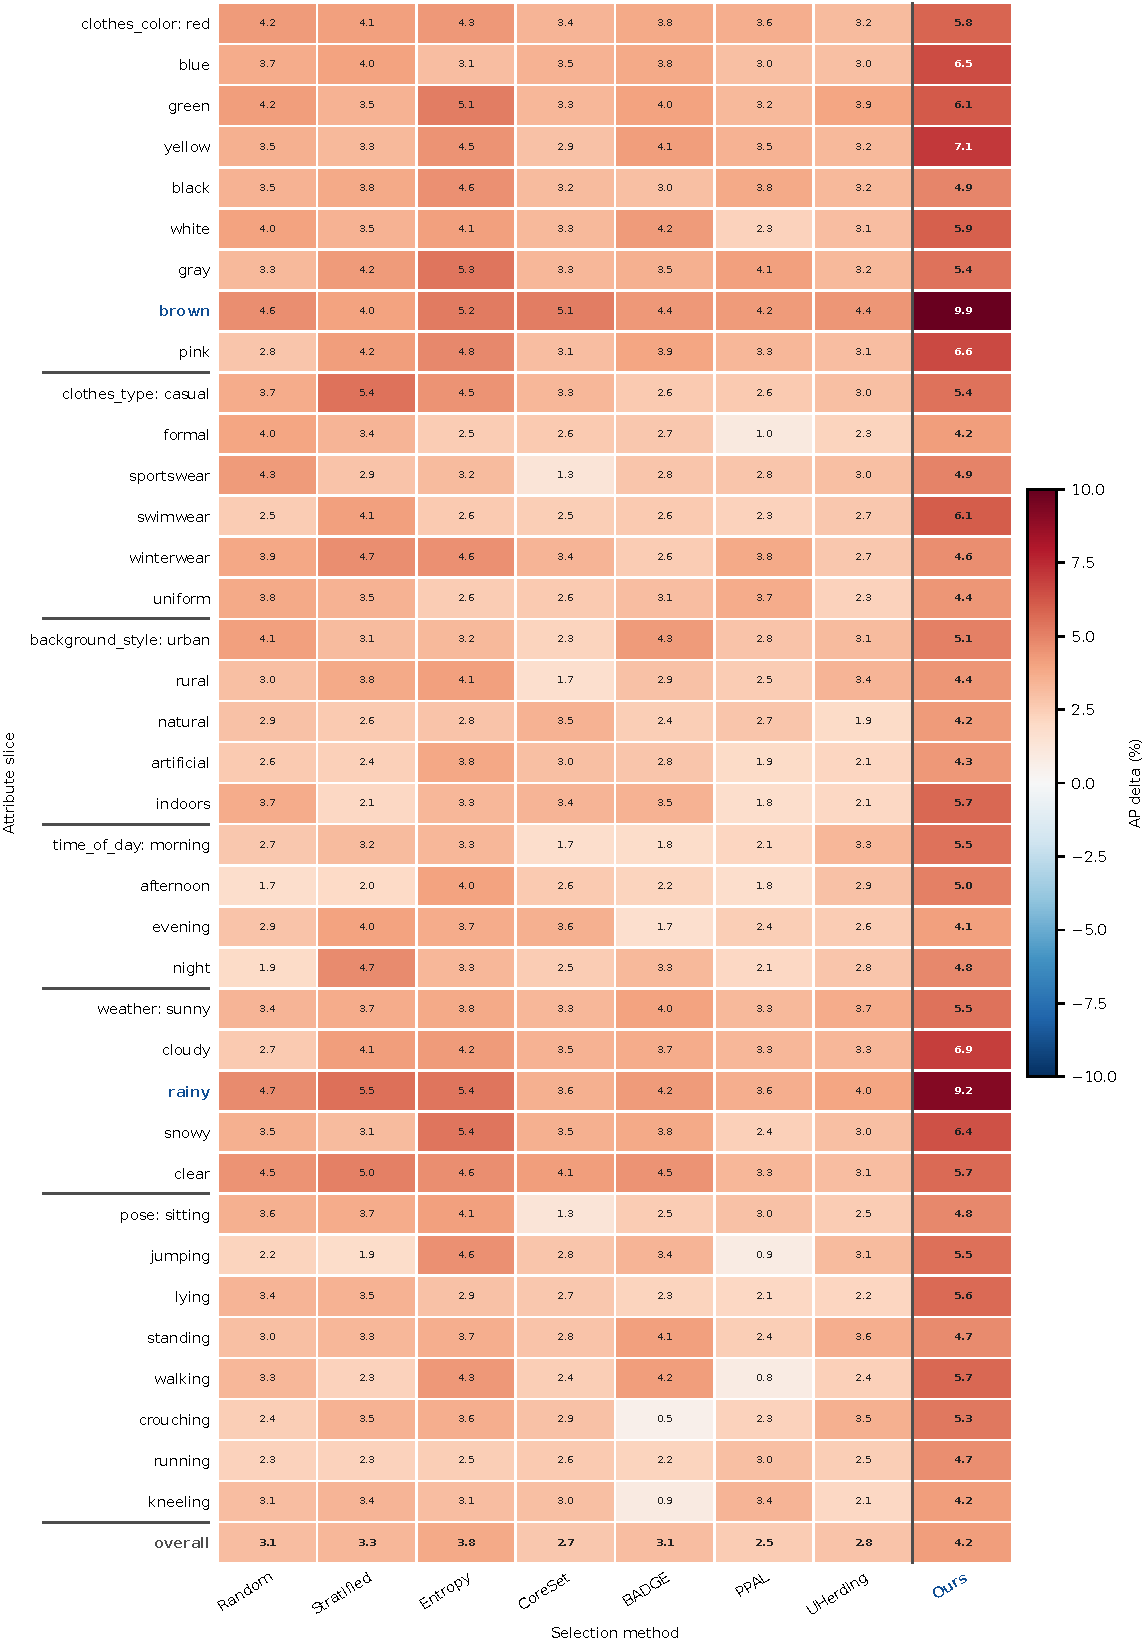
\includegraphics[width=\linewidth]{figures/show/coco_ratio0p5_show_heatmap.pdf}
\caption{COCO pose-estimation ratio-$0.5$ attribute-slice AP deltas. The figure expands the slice-level analysis to all annotated COCO pose-estimation attribute groups. The targeted repair values are clothes color brown and rainy weather.}
\label{fig:coco-ratio05-attribute-delta}
\end{figure}


\section{Effect of the VLM and Human Audit}
\label{app:vlm-human-audit}

\paragraph{VLM Role and Leakage Control}
\textbf{Where VLM annotations enter.}
\model uses the VLM as a fixed attribute annotator. Given a task-specific set of attribute fields and closed-set label options, the VLM assigns a discrete value to each image. The selector then uses these values, class labels, and generated-data attribute counts to choose the source subset. The repair-slice indicator is the binary conjunction of the target attribute values for the corresponding task: red hair, brown skin, and sad emotion for CelebA; pink color and fabric texture for ImageNet10; brown clothes and rainy weather for COCO; and red object color and cloudy weather for KITTI. The main repair metrics in Tables~\ref{tab:main-fr} and~\ref{tab:app-main-imagenet}--\ref{tab:app-main-kitti} are standard task metrics computed from benchmark labels, so the VLM does not grade the final repaired model. Test-set attributes are used only for post-training slice diagnostics.

\vspace{0.5em}
\textbf{Leakage control.}
The attribute vocabulary, target fields, and VLM annotation prompt are fixed before running the source-selection methods. The assignment stage does not receive model predictions, failure rates, method names, selected-set membership, or downstream results. In settings where the same VLM family is used for target-slice wording and image-level assignment, the two roles are still separated: the slice description is fixed first, and assignment is then run as a frozen closed-set classifier over images. Source selection uses only source-training attributes and generated-pool attributes. Thus a possible failure mode is not test-label leakage, but inaccurate or self-consistent metadata. The audit below tests the target fields with independent human labels.

\paragraph{Human Audit Protocol}
We conduct a blinded human audit with five AI graduate students. Each annotator labels 100 CelebA images, 100 COCO images, and 100 KITTI images using the same closed-set options as the VLM. Annotators see only the image, dataset name, and sample identifier; they do not see VLM labels, target flags, model predictions, data split, or method outputs. We aggregate human labels by majority vote and compare them with the VLM labels at two levels: exact agreement on the audited fields and binary agreement on the repair-slice indicator after applying the target values for those fields. For example, the COCO slice indicator is true only when the audited image has brown clothes and rainy weather, and the KITTI indicator is true only when it has red object color and cloudy weather. For CelebA, the indicator uses the full repair conjunction over red hair, brown skin, and sad emotion, rather than a single field such as hair color alone. The binary agreement is the most relevant check for \model because the selector uses these attributes to identify repair-relevant source examples.

\begin{table}[h]
\centering
\caption{Human audit of VLM-assigned attributes. Five AI graduate students label each audited image using the same closed-set options as the VLM. Exact field agreement measures agreement on the audited attribute values, while slice-indicator agreement measures agreement on the binary target conjunction used for repair.}
\label{tab:vlm-human-audit}
\small
\setlength{\tabcolsep}{3pt}
\begin{tabular}{p{0.14\linewidth} C{0.27\linewidth} C{0.27\linewidth} C{0.22\linewidth}}
\toprule
\rowcolor{sectiongray} \textbf{Dataset} & \textbf{Target field 1 agree.} & \textbf{Target field 2 agree.} & \textbf{Slice-indicator agree.} \\
\midrule
CelebA & Hair color: 98\% & Skin tone: 99\% & 92\% \\
COCO & Clothes color: 97\% & Weather: 91\% & 90\% \\
KITTI & Object color: 98\% & Weather: 96\% & 94\% \\
\bottomrule
\end{tabular}
\end{table}

The audit is designed to measure agreement rather than to estimate the prevalence of rare target conjunctions. As shown in Table~\ref{tab:vlm-human-audit}, the VLM and human consensus usually agree on the audited target fields and on the resulting binary slice indicators. This supports the use of the VLM as a scalable attribute annotator rather than as an oracle: the VLM provides metadata, and the human audit checks that the target fields used for repair are visually grounded.

\paragraph{Sensitivity to attribute noise.}
We also test whether \model is brittle to noisy attributes. For each audited dataset and each target field, we independently corrupt a fraction $p$ of VLM labels by replacing the original value with a different valid value from the same field vocabulary. We then rerun source selection with the corrupted attributes while keeping the generated repair set, source ratio, and training recipe fixed. Table~\ref{tab:attribute-noise-sensitivity} reports the change from the clean-VLM \model result at source ratio $0.5$ for CelebA, COCO, and KITTI. Small changes under moderate noise would indicate that the selector depends on the aggregate attribute distribution rather than on a small number of individual VLM decisions.

\begin{table}[h]
\centering
\caption{Sensitivity to corrupted VLM attributes at source ratio $0.5$. Entries report the change from the clean-VLM \model result for each task metric.}
\label{tab:attribute-noise-sensitivity}
\small
\setlength{\tabcolsep}{5pt}
\begin{tabular}{l c c c c}
\toprule
\rowcolor{sectiongray} \textbf{Dataset} & \textbf{Metric} & \textbf{5\% noise} & \textbf{10\% noise} & \textbf{20\% noise} \\
\midrule
CelebA & Test ACC $\Delta$ & 0.007 & 0.01 & 0.09 \\
COCO & Test AP $\Delta$ & 0.002 & 0.003 & 0.02 \\
KITTI & Test mAP50--95 $\Delta$ & 0.003 & 0.004 & 0.06 \\
\bottomrule
\end{tabular}
\end{table}

The results show that \model is relatively stable to light and moderate attribute noise. At $5\%$ and $10\%$ corruption, the metric changes are small across all three datasets, which suggests that the selector is not driven by a few isolated attribute assignments. The larger shifts at $20\%$ noise, especially on CelebA and KITTI, are expected: once many target-field labels are replaced, the rarity and frequency counts no longer describe the diagnosed repair slice reliably. In this high-noise regime, \model no longer behaves like a clean semantic selector. Its ranking is partly driven by corrupted attribute values, while the soft class-balance term still preserves label coverage, so the selected subset moves toward a mixture of noisy attribute sampling and soft stratified sampling. This explains why the results begin to approach the behavior of random or stratified source selection when the attribute metadata is heavily corrupted. COCO is less sensitive in this range, suggesting that its selected subset is more strongly supported by aggregate attribute statistics or by other correlated visual factors in the source pool.


\section{Effect of Image Generation}
\label{app:image-generation-effect}

The upstream workflow following \safefix~\citep{xu2025safefix} uses \controlnet~\citep{zhang2023adding} as the conditional diffusion model. The quality of diffusion-based dataset augmentation can vary with the generator and editing procedure~\citep{trabucco2023effective,dunlap2023diversify,wang2024domain}. To test whether \model depends on this particular generator, we replace \controlnet while keeping the rest of the repair pipeline fixed: InstructPix2Pix~\citep{brooks2023instructpix2pix} for CelebA and ICEdit~\citep{zhang2025icedit} for COCO.

Table~\ref{tab:celeba-instructpix2pix-fr} reports CelebA results with InstructPix2Pix generation. \model remains the strongest source selector at every active source ratio. Its absolute FR is lower than the corresponding \controlnet result in Table~\ref{tab:main-fr}, but the same decrease is visible across the other selectors, indicating that this shift comes from the generated repair images rather than from the source-selection rule.

\begin{table}[h]
\centering
\caption{CelebA repair results with InstructPix2Pix generation. Metric: FR (\%).}
\label{tab:celeba-instructpix2pix-fr}
\footnotesize
\setlength{\tabcolsep}{3pt}
\begin{tabular}{c c c c c c c c >{\columncolor{myblue!8}}c | >{\columncolor{myblue!8}}c}
\toprule
\rowcolor{sectiongray} \textbf{Ratio} & \textbf{Random} & \textbf{Stratified} & \textbf{Entropy} & \textbf{CoreSet} & \textbf{BADGE} & \textbf{UHerding} & \textbf{PPAL} & \cellcolor{myblue!8}\textbf{Ours (InstructPix2Pix)} & \cellcolor{myblue!8}\textbf{Ours (ControlNet)} \\
\midrule
0.1 & 4.23 & 1.95 & 6.41 & -6.65 & 2.34 & -1.78 & 5.12 & \textbf{7.65} & 8.48 \\
0.3 & 5.34 & 4.72 & 7.98 & 7.21 & 1.02 & 2.81 & 3.45 & \textbf{8.12} & 8.91 \\
0.5 & 5.56 & 7.23 & 6.78 & 7.54 & 2.12 & 1.56 & 9.12 & \textbf{11.17} & 13.79 \\
0.7 & 2.12 & 7.67 & 9.34 & 5.78 & 7.34 & 4.23 & 5.34 & \textbf{12.13} & 12.09 \\
0.9 & 2.45 & 3.92 & 7.56 & 5.34 & 5.23 & 3.87 & 5.91 & \textbf{13.87} & 14.74 \\
\bottomrule
\end{tabular}
\end{table}

Table~\ref{tab:coco-icedit-fr} reports the corresponding COCO result with ICEdit. ICEdit improves the absolute FR values for most source ratios, and \model remains the best selector under this generator as well. These comparisons should be read horizontally: for a fixed generator and generated repair set, \model is compared against the non-attribute active-learning selectors. Changes in generator quality can shift the absolute repair numbers, but they do not remove the benefit of attribute-driven source selection.

\begin{table}[h]
\centering
\caption{COCO pose-estimation repair results with ICEdit generation. Metric: FR (\%).}
\label{tab:coco-icedit-fr}
\footnotesize
\setlength{\tabcolsep}{3pt}
\begin{tabular}{c c c c c c c c >{\columncolor{myblue!8}}c | >{\columncolor{myblue!8}}c}
\toprule
\rowcolor{sectiongray} \textbf{Ratio} & \textbf{Random} & \textbf{Stratified} & \textbf{Entropy} & \textbf{CoreSet} & \textbf{BADGE} & \textbf{UHerding} & \textbf{PPAL} & \cellcolor{myblue!8}\textbf{Ours (ICEdit)} & \cellcolor{myblue!8}\textbf{Ours (ControlNet)} \\
\midrule
0.1 & 3.78 & 5.23 & 5.87 & -0.34 & 2.34 & 3.12 & 1.56 & \textbf{7.12} & 6.86 \\
0.3 & 3.92 & 8.67 & 8.12 & 9.12 & 6.56 & 4.67 & 6.89 & \textbf{10.34} & 9.86 \\
0.5 & 7.91 & 8.45 & 9.67 & 6.91 & 7.82 & 6.54 & 7.23 & \textbf{10.67} & 10.13 \\
0.7 & 6.54 & 10.12 & 9.98 & 9.56 & 9.12 & 6.71 & 8.23 & \textbf{10.87} & 10.18 \\
0.9 & 5.12 & 9.87 & 6.98 & 7.82 & 8.12 & 7.54 & 10.12 & \textbf{11.56} & 11.05 \\
\bottomrule
\end{tabular}
\end{table}


\section{Additional Theory Analysis}
\label{app:theory-analysis}

\paragraph{Slice enrichment}
We use \emph{slice enrichment} to describe whether a selected source subset contains more examples from the diagnosed target slice than would be expected from its class-conditional base rate.

\begin{tcolorbox}[
    colback=blue!2!white,
    colframe=blue!20!white,
    arc=3pt,
    boxrule=1pt,
    drop shadow,
    breakable
]
\textbf{Proposition 1 (Attribute-agnostic AL requires target alignment).} \textit{Consider any AL selector that, within class $c$, chooses $B_c$ source examples using only non-attribute information $h_i$, such as uncertainty, logits, embeddings, losses, detector difficulty, coverage, or image distances, and does not use the attribute values $\{v_{i,a}:a\in\attrs\}$. Let $\dataset_{\mathrm{AL}}$ denote its selected source subset. If the target-slice indicator $\mathbf{1}[x_i\in T_c]$ is conditionally independent of $h_i$ given class $c$, with ties and internal randomness independent of the target indicator, then
\begin{equation*}
\mathbb{E}\big[|\dataset_{\mathrm{AL}}\cap T_c|\big]
=
B_c\frac{|T_c|}{N_c}.
\end{equation*}
Thus an attribute-agnostic AL method can enrich the target slice only when its non-attribute signal is additionally aligned with that slice.}
\end{tcolorbox}

\begin{tcolorbox}[
    colback=green!2!white,
    colframe=green!20!white,
    arc=3pt,
    boxrule=1pt,
    drop shadow,
    breakable
]
\begin{proof}[Proof of Proposition~\ref{prop:al-target-alignment}]
Conditional independence makes the target indicators exchangeable with respect to any ranking, batch construction, or randomized choice computed from $h_i$ inside class $c$. The $B_c$ selected positions therefore contain, in expectation, the same target-slice fraction as the class pool itself, namely $|T_c|/N_c$. This argument does not depend on the particular AL heuristic. Uncertainty sampling, margin sampling, loss-based selection, diversity sampling, CoreSet, BADGE, PPAL-style uncertainty-then-diversity selection, and Uncertainty Herding-style uncertainty coverage all fall under the claim whenever their selection variables omit the current attribute metadata and are not otherwise aligned with the target slice.

As a concrete coverage-based instance, let $z_i$ be the representation used by a diversity or coverage selector, such as cluster-based Diversity, CoreSet in feature space, or BADGE in gradient-embedding space. CoreSet-style $k$-center selection minimizes
\begin{equation}
\label{eq:k-center-objective}
\max_i \min_{j\in S} d(z_i,z_j),
\end{equation}
so achieving objective value at most $\epsilon$ is equivalent to constructing an $\epsilon$-cover of the source representations. For a finite set $A$ in this representation space, define the empirical covering number
\begin{equation}
\label{eq:empirical-covering-number}
\mathcal{N}^{\mathrm{emp}}_{\epsilon}(A)
=
\min\big\{|C|: C\subseteq A,\; A\subseteq \cup_{z\in C}B(z,\epsilon)\big\}.
\end{equation}
If the target slice in class $c$ has empirical covering number
\begin{equation}
\label{eq:target-covering-number}
q_c=\mathcal{N}^{\mathrm{emp}}_{\epsilon}\big(\{z_i:x_i\in T_c\}\big),
\end{equation}
then an $\epsilon$-cover objective can cover the entire target region using only $q_c$ selected target representatives. Consequently, when the non-target region still contains uncovered $\epsilon$-scale cells, a coverage-based selector has an optimal solution with at most $q_c$ selected target examples, even if $|T_c|\gg q_c$.

For this coverage-based instance, take $h_i=z_i$. By definition of the empirical covering number, there exists a subset $C_T\subseteq \{z_i:x_i\in T_c\}$ with $|C_T|=q_c$ such that every target-slice representation is within distance $\epsilon$ of some point in $C_T$. Selecting the corresponding $q_c$ target examples therefore makes the whole target slice $\epsilon$-covered. Any additional target example only refines coverage inside an already covered target region. If non-target $\epsilon$-scale cells remain uncovered, a coverage or diversity objective can spend the remaining representatives outside $T_c$ without increasing its maximum covering radius. Thus feature-space coverage does not force more than $q_c$ target selections.

The same conclusion follows from the usual volumetric intuition. If a class region has effective dimension $d$, volume $V$, and the target subregion has volume $V_T$, then away from boundary effects an $\epsilon$-cover requires on the order of $V/(v_d\epsilon^d)$ cells for the full class region but only $V_T/(v_d\epsilon^d)$ cells for the target region, where $v_d$ is the volume of the unit $d$-ball. When the bug slice is semantically important but geometrically compact, $V_T\ll V$, so the number of representatives allocated by a geometry-only objective can be small. The objective allocates capacity to representation volume, not to semantic repair importance.
\end{proof}
\end{tcolorbox}

\paragraph{Rarity and generated-data penalty}
We now show why the attribute score assigns strict priority to a rare target slice under explicit data conditions. For any target example $x_i\in T_c$ and non-target example $x_j\notin T_c$ from the same class $c$, define the attributes on which they differ as
\begin{equation}
\label{eq:target-difference-attributes}
\mathcal{D}_{ij}=\{a\in\attrs: v_{i,a}\neq v_{j,a}\}.
\end{equation}
Let
\begin{equation}
\label{eq:rarity-advantage}
A_{ij}
=
\sum_{a\in\mathcal{D}_{ij}}
\left[
\left(\frac{1}{n_a(v_{i,a}\mid c)+\varepsilon}\right)^\alpha
-
\left(\frac{1}{n_a(v_{j,a}\mid c)+\varepsilon}\right)^\alpha
\right]
\end{equation}
be the rarity advantage of the target example, and let
\begin{equation}
\label{eq:frequency-disadvantage}
F_{ij}
=
\sum_{a\in\mathcal{D}_{ij}}
\left[
\frac{\hat{n}_a(v_{i,a})}{\sum_{v\in\vals_a}\hat{n}_a(v)}
-
\frac{\hat{n}_a(v_{j,a})}{\sum_{v\in\vals_a}\hat{n}_a(v)}
\right]
\end{equation}
be the frequency-penalty disadvantage introduced by source and generated counts. If generated data has flooded the target value, then $F_{ij}$ can be positive; if not, the penalty does not hurt the target example relative to $x_j$.

\begin{tcolorbox}[
    colback=blue!2!white,
    colframe=blue!20!white,
    arc=3pt,
    boxrule=1pt,
    drop shadow,
    breakable
]
\begin{proposition}[Rarity-dominates-penalty margin]
\label{prop:rarity-margin}
Assume $\alpha>0$ and $A_{ij}>0$ for every target/non-target pair $(x_i,x_j)$ within class $c$. Define
\begin{equation}
\label{eq:lambda-star}
\lambda_c^\star
=
\min_{x_i\in T_c,\;x_j\notin T_c,\;F_{ij}>0}
\frac{A_{ij}}{F_{ij}},
\end{equation}
with $\lambda_c^\star=\infty$ if no pair has $F_{ij}>0$. For any $0\leq\lambda<\lambda_c^\star$, every target example in $T_c$ has larger base score $\bar{s}_i$ than every non-target example from the same class. In particular, when each target attribute value is rarer than the competing non-target value, i.e., $n_a(v_{i,a}\mid c)<n_a(v_{j,a}\mid c)$ for all $a\in\mathcal{D}_{ij}$, the condition $A_{ij}>0$ holds automatically.
\end{proposition}
\end{tcolorbox}

\begin{tcolorbox}[
    colback=green!2!white,
    colframe=green!20!white,
    arc=3pt,
    boxrule=1pt,
    drop shadow,
    breakable
]
\begin{proof}
For a target/non-target pair $(x_i,x_j)$ in class $c$, attributes outside $\mathcal{D}_{ij}$ contribute the same score to both examples and cancel. The remaining base-score gap is
\begin{equation}
\label{eq:base-score-gap}
\bar{s}_i-\bar{s}_j
=
A_{ij}-\lambda F_{ij}.
\end{equation}
If $F_{ij}\leq 0$, then $\bar{s}_i-\bar{s}_j\geq A_{ij}>0$ for any $\lambda\geq 0$, so the frequency penalty does not overturn the rarity advantage. If $F_{ij}>0$, then $\bar{s}_i-\bar{s}_j>0$ whenever $\lambda<A_{ij}/F_{ij}$. Taking the minimum over all target/non-target pairs with $F_{ij}>0$ gives the interval $0\leq\lambda<\lambda_c^\star$, under which every pair has a strictly positive score gap. Finally, if $n_a(v_{i,a}\mid c)<n_a(v_{j,a}\mid c)$ and $\alpha>0$, then each rarity term in $A_{ij}$ is positive, so their sum is positive.
\end{proof}
\end{tcolorbox}

This proposition is the main data-dependent guarantee. It says that if the VLM annotations correctly identify a genuinely rare target slice, then there is a nonempty range of $\lambda$ values for which rarity dominates the synthetic-data frequency penalty. Even when generated examples make the target value more frequent in the repair candidate pool, the target examples remain ranked above non-target examples as long as $\lambda$ is below the explicit threshold $\lambda_c^\star$. Conversely, if target and non-target samples are indistinguishable under $\attrs$, then no attribute-only selector can separate them without additional information.

\begin{tcolorbox}[
    colback=blue!2!white,
    colframe=blue!20!white,
    arc=3pt,
    boxrule=1pt,
    drop shadow,
    breakable
]
\begin{proposition}[Deterministic rare-slice enrichment]
\label{prop:deterministic-enrichment}
Assume the rarity-dominates-penalty condition in Proposition~\ref{prop:rarity-margin} holds for class $c$ and the $\lambda$ used by the selector. If the class-aware re-ranking step allocates $B_c$ source samples to class $c$, then \model includes at least
\begin{equation}
\label{eq:deterministic-enrichment-bound}
\min\{B_c,|T_c|\}
\end{equation}
target-slice examples from that class. A random or stratified selector with the same class allocation selects
\begin{equation}
\label{eq:random-target-expectation}
\mathbb{E}\big[|S_{\mathrm{rand}}\cap T_c|\big]
=
B_c\frac{|T_c|}{N_c}
\end{equation}
target examples in expectation.
\end{proposition}
\end{tcolorbox}

\begin{tcolorbox}[
    colback=green!2!white,
    colframe=green!20!white,
    arc=3pt,
    boxrule=1pt,
    drop shadow,
    breakable
]
\begin{proof}
At a fixed greedy step, the class-aware term adds the same bonus $\textcolor{colorC}{C_c^{(k)}}$ to every remaining candidate from class $c$. Therefore it can change how many samples are selected from each class, but it cannot reverse the within-class ordering induced by the base attribute score $\bar{s}_i$. By Proposition~\ref{prop:rarity-margin}, all target-slice examples in class $c$ appear before all non-target examples in the class queue. Selecting $B_c$ samples from that queue must therefore include all target examples when $|T_c|\leq B_c$, and $B_c$ target examples when $|T_c|>B_c$. This proves the deterministic bound. For random or stratified sampling under the same class allocation, each selected class-$c$ source example has probability $|T_c|/N_c$ of belonging to the target slice, giving the expectation by linearity.
\end{proof}
\end{tcolorbox}

The enrichment gap is strict whenever $0<|T_c|<N_c$ and $B_c>0$, because
\begin{equation}
\label{eq:enrichment-gap}
\min\{B_c,|T_c|\}\geq B_c\frac{|T_c|}{N_c}.
\end{equation}
Thus \model provides a semantic coverage guarantee for the repair surrogate, while random, stratified, uncertainty, Diversity, CoreSet, BADGE, PPAL, and Uncertainty Herding require additional alignment between their selection signal and the target slice.

\begin{tcolorbox}[
    colback=blue!2!white,
    colframe=blue!20!white,
    arc=3pt,
    boxrule=1pt,
    drop shadow,
    breakable
]
\begin{proposition}[Uncertainty can miss an attribute slice]
Consider uncertainty-based selection within each class, with uncertainty score $Q_i$ and class allocation $B_c$. If the $B_c$ largest uncertainty scores among non-target examples in class $c$ are all larger than every uncertainty score in $T_c$, then uncertainty selection chooses zero examples from $T_c$.
\end{proposition}
\end{tcolorbox}

\begin{tcolorbox}[
    colback=green!2!white,
    colframe=green!20!white,
    arc=3pt,
    boxrule=1pt,
    drop shadow,
    breakable
]
\begin{proof}
The claim is deterministic. If at least $B_c$ non-target examples have uncertainty larger than every target example, the top-$B_c$ uncertainty set contains only non-target examples. The same argument applies to any two-stage uncertainty-first method when the first-stage pool contains no target-slice examples: no second-stage diversity or coverage rule can recover target support that is absent from its candidate pool.
\end{proof}
\end{tcolorbox}

Finally, suppose the repair utility of a selected source subset is
\begin{equation}
\label{eq:repair-utility}
U(S)=u_0 |S| + (u_T-u_0)|S\cap T|,
\qquad u_T>u_0,
\end{equation}
meaning target-slice samples have larger marginal value for the discovered repair problem. Then the rare-slice enrichment bound directly implies expected utility at least as large as random or stratified selection under the same class allocation, with a strict gap whenever the enrichment gap is strict. This is not a universal proof that the final trained model must dominate every baseline for every ratio; it is a conditional guarantee that the selector spends a fixed budget on more repair-relevant examples when the VLM metadata and count conditions correctly identify the failing slice.

\paragraph{Soft class-balance behavior}
The enrichment result above is within-class: the soft class-balance term changes how many examples are drawn from each class, but it does not reverse the attribute ordering inside a class. The following two results summarize the role of $C$.

\begin{tcolorbox}[
    colback=blue!2!white,
    colframe=blue!20!white,
    arc=3pt,
    boxrule=1pt,
    drop shadow,
    breakable
]
\begin{proposition}[Hard-balance limit]
\label{prop:hard-balance-limit}
When $w=\infty$ and every active class has enough candidates, the round-robin limit selects class counts that differ by at most one. Within each class, candidates are still ordered by the attribute score $\bar{s}_i$.
\end{proposition}
\end{tcolorbox}

\begin{tcolorbox}[
    colback=green!2!white,
    colframe=green!20!white,
    arc=3pt,
    boxrule=1pt,
    drop shadow,
    breakable
]
\begin{proof}
The round-robin rule visits one active class at a time and removes the highest-scoring remaining candidate from that class. After each visit, the class is moved to the back of the queue. Thus no class can receive a second additional sample before every other non-empty class has received one. The selected counts across non-empty classes therefore differ by at most one, except when a class runs out of candidates. Since each class queue is sorted by $\bar{s}_i$, the within-class attribute order is preserved.
\end{proof}
\end{tcolorbox}

\begin{tcolorbox}[
    colback=blue!2!white,
    colframe=blue!20!white,
    arc=3pt,
    boxrule=1pt,
    drop shadow,
    breakable
]
\begin{proposition}[Finite-weight balance pressure]
\label{prop:finite-weight-balance}
Assume $0<w<\infty$. At greedy step $k$, let $A_c^{(k)}$ be the highest remaining base score in class $c$, and assume all active class-head scores lie in an interval of width
\begin{equation}
\label{eq:class-head-width}
\Delta = \max_c A_c^{(k)} - \min_c A_c^{(k)}.
\end{equation}
If class $d$ is selected at step $k$ while another class $c$ is also active, then
\begin{equation}
\label{eq:finite-balance-gap}
n_d^{(k)} - n_c^{(k)} \leq \frac{t\Delta}{w}.
\end{equation}
Equivalently, if an active class $c$ trails class $d$ by more than $t\Delta/w$, then class $d$ cannot be selected before class $c$ at that step.
\end{proposition}
\end{tcolorbox}

\begin{tcolorbox}[
    colback=green!2!white,
    colframe=green!20!white,
    arc=3pt,
    boxrule=1pt,
    drop shadow,
    breakable
]
\begin{proof}
Since class $d$ is selected, its adjusted score is at least the adjusted score of class $c$:
\begin{equation}
\label{eq:finite-balance-proof-start}
A_d^{(k)} + w\frac{t-n_d^{(k)}}{t}
\geq
A_c^{(k)} + w\frac{t-n_c^{(k)}}{t}.
\end{equation}
Rearranging gives
\begin{equation}
\label{eq:finite-balance-proof-rearranged}
\frac{w}{t}\big(n_d^{(k)}-n_c^{(k)}\big)
\leq A_d^{(k)}-A_c^{(k)}.
\end{equation}
Because both class-head scores lie in an interval of width $\Delta$, we have $A_d^{(k)}-A_c^{(k)}\leq\Delta$. Therefore $n_d^{(k)}-n_c^{(k)}\leq t\Delta/w$.
\end{proof}
\end{tcolorbox}

This finite-weight result gives the exact sense in which $w$ controls soft balance. When $w=0$, the bound disappears and the selector reduces to pure attribute ranking. When $0<w<\infty$, a class with a large deficit receives enough bonus to overcome any bounded attribute-score advantage from an over-selected class. Increasing $w$ tightens the admissible count gap by the factor $1/w$. In the limiting case $w\rightarrow\infty$, the admissible gap goes to zero, matching the round-robin behavior in Proposition~\ref{prop:hard-balance-limit}. Thus finite $w$ does not guarantee exact class quotas, but it guarantees that class imbalance can persist only when the over-selected class has a sufficiently larger attribute score at the current step.

\subsection{No-Generation Corner Case}
\label{app:no-generation-corner-case}

This section discusses the corner case in which no generated repair images are available, i.e., $\dataset_{\mathrm{gen}}=\emptyset$. This setting removes the main mechanism for adding missing semantic support, but \model still has a useful source-selection interpretation. Since $\tilde{n}_a^{\mathrm{gen}}(v)=0$, the effective count becomes
\begin{equation}
\hat{n}_a(v)=n_a^{\mathrm{src}}(v),
\end{equation}
and the base score reduces to
\begin{equation}
\bar{s}_i
=
\sum_{a \in \attrs}
\left[
\left(\frac{1}{n_a(v_{i,a}\mid y_i)+\varepsilon}\right)^\alpha
-
\lambda
\frac{n_a^{\mathrm{src}}(v_{i,a})}{\sum_{v\in\vals_a} n_a^{\mathrm{src}}(v)}
\right].
\end{equation}
Thus, when $\dataset_{\mathrm{gen}}=\emptyset$, the frequency penalty is no longer correcting a synthetic flood. It becomes a source-distribution head-value penalty: values that are already common in the source pool receive lower priority. The rarity term still prefers values that are rare within a class, and the soft class-balance term still controls label-level collapse.

\begin{tcolorbox}[
    colback=blue!2!white,
    colframe=blue!20!white,
    arc=3pt,
    boxrule=1pt,
    drop shadow,
    breakable
]
\begin{proposition}[Source-only rare-slice enrichment]
Let $\dataset_{\mathrm{gen}}=\emptyset$ and let $T\subseteq\dataset_{\mathrm{src}}$ be a target failure slice with nonzero source support. Suppose the rarity-dominates-penalty condition in Proposition~\ref{prop:rarity-margin} holds for $T$ under the source-only score above, with $\hat{n}_a(v)=n_a^{\mathrm{src}}(v)$. If the class-aware re-ranking step selects $B_c$ samples from class $c$, then \model returns at least
\begin{equation}
\sum_c \min\{B_c, |T_c|\}
\end{equation}
source examples from $T$. A random selector with the same per-class allocation selects
\begin{equation}
\mathbb{E}\big[|S_{\mathrm{rand}}\cap T|\big]
=
\sum_c B_c\frac{|T_c|}{N_c}
\end{equation}
target-slice examples in expectation.
\end{proposition}
\end{tcolorbox}

\begin{tcolorbox}[
    colback=green!2!white,
    colframe=green!20!white,
    arc=3pt,
    boxrule=1pt,
    drop shadow,
    breakable
]
\begin{proof}
The proof is identical to the rare-slice enrichment proof in Appendix~\ref{app:theory-analysis}, because that argument uses only the within-class ordering induced by $\bar{s}_i$. When $\dataset_{\mathrm{gen}}=\emptyset$, the score changes only through the replacement $\hat{n}_a(v)=n_a^{\mathrm{src}}(v)$. If the source-only score satisfies the rarity-dominates-penalty condition, then all target-slice samples appear before non-target samples in each class queue. Selecting $B_c$ examples from class $c$ therefore includes $\min\{B_c,|T_c|\}$ target examples. The random expectation follows by linearity under sampling from each class with allocation $B_c$.
\end{proof}
\end{tcolorbox}

This proposition shows that generation is not required for the selector to improve target-slice coverage when the source pool already contains target examples. In this regime, the method becomes semantic active subset selection over the source pool. It can increase the number of existing rare failure cases in the retraining subset, but it cannot create support for a target slice that is absent from the source pool.

\begin{tcolorbox}[
    colback=blue!2!white,
    colframe=blue!20!white,
    arc=3pt,
    boxrule=1pt,
    drop shadow,
    breakable
]
\begin{proposition}[Impossibility for absent source slices]
Let $\dataset_{\mathrm{gen}}=\emptyset$ and suppose $T\cap\dataset_{\mathrm{src}}=\emptyset$. Then every source-only selector $S\subseteq\dataset_{\mathrm{src}}$ satisfies
\begin{equation}
|S\cap T|=0.
\end{equation}
Consequently, no active-selection rule over $\dataset_{\mathrm{src}}$ alone can provide target-slice training support.
\end{proposition}
\end{tcolorbox}

\begin{tcolorbox}[
    colback=green!2!white,
    colframe=green!20!white,
    arc=3pt,
    boxrule=1pt,
    drop shadow,
    breakable
]
\begin{proof}
Since $S\subseteq\dataset_{\mathrm{src}}$ and $T\cap\dataset_{\mathrm{src}}=\emptyset$, we have $S\cap T\subseteq\dataset_{\mathrm{src}}\cap T=\emptyset$. Hence $|S\cap T|=0$ for every possible selector.
\end{proof}
\end{tcolorbox}

The no-generation case therefore separates two roles of \model. If $T$ already appears in the source pool, attribute selection can enrich those existing target examples under the same rarity-dominates-penalty condition as the main result. If $T$ is absent from the source pool, selection alone is insufficient; repair requires either new data collection or generated images that add target-slice support. This also clarifies the role of $\lambda$: with no generated images, a large frequency penalty may suppress globally common values even when they are rare within a specific class. In source-only repair, $\lambda$ should therefore be interpreted as a head-value suppression weight and may need to be smaller than in settings with heavy generated-data injection.

\section{Main-Result Metric Tables}
\label{app:main-metric-tables}

This section reports the original task metrics corresponding to the Fix Rate tables in the main text. The metrics are test accuracy for ImageNet10 and CelebA, COCO keypoint AP for pose estimation, and test mAP50--95 for KITTI object detection. All entries report the mean and standard deviation ($\pm$) over seeds 0, 42, 1234, 3407, and 2024. We performed paired t-tests to evaluate statistical significance, confirming that the improvements of \model over the respective best baselines are statistically significant ($p < 0.05$) across the reported selection ratios.

\begin{table}[h]
\centering
\caption{ImageNet10 classification repair results. Metric: test accuracy.}
\label{tab:app-main-imagenet}
\small
\setlength{\tabcolsep}{3pt}
\resizebox{\linewidth}{!}{%
\begin{tabular}{c c c c c c c c >{\columncolor{myblue!8}}c}
\toprule
\rowcolor{sectiongray} \textbf{Ratio} & \textbf{Random} & \textbf{Stratified} & \textbf{Entropy} & \textbf{CoreSet} & \textbf{BADGE} & \textbf{UHerding} & \textbf{PPAL} & \cellcolor{myblue!8}\textbf{Ours} \\
\midrule
0.1 & 0.7269$_{\pm 0.0025}$ & 0.7271$_{\pm 0.0037}$ & 0.7254$_{\pm 0.0016}$ & 0.7269$_{\pm 0.0032}$ & 0.7323$_{\pm 0.0022}$ & 0.7331$_{\pm 0.0023}$ & 0.7285$_{\pm 0.0026}$ & \textbf{0.7369$_{\pm 0.0043}$} \\
0.3 & 0.7308$_{\pm 0.0020}$ & 0.7369$_{\pm 0.0036}$ & 0.7292$_{\pm 0.0016}$ & 0.7369$_{\pm 0.0012}$ & 0.7423$_{\pm 0.0036}$ & 0.7469$_{\pm 0.0043}$ & 0.7392$_{\pm 0.0022}$ & \textbf{0.7492$_{\pm 0.0044}$} \\
0.5 & 0.7380$_{\pm 0.0030}$ & 0.7446$_{\pm 0.0017}$ & 0.7331$_{\pm 0.0027}$ & 0.7400$_{\pm 0.0017}$ & 0.7469$_{\pm 0.0029}$ & 0.7410$_{\pm 0.0028}$ & 0.7423$_{\pm 0.0016}$ & \textbf{0.7508$_{\pm 0.0010}$} \\
0.7 & 0.7423$_{\pm 0.0043}$ & 0.7346$_{\pm 0.0043}$ & 0.7354$_{\pm 0.0042}$ & 0.7392$_{\pm 0.0043}$ & 0.7477$_{\pm 0.0011}$ & 0.7469$_{\pm 0.0034}$ & 0.7423$_{\pm 0.0034}$ & \textbf{0.7515$_{\pm 0.0037}$} \\
0.9 & 0.7462$_{\pm 0.0040}$ & 0.7469$_{\pm 0.0011}$ & 0.7462$_{\pm 0.0026}$ & 0.7346$_{\pm 0.0035}$ & 0.7438$_{\pm 0.0027}$ & 0.7500$_{\pm 0.0033}$ & 0.7508$_{\pm 0.0041}$ & \textbf{0.7562$_{\pm 0.0019}$} \\
\noalign{\vskip 1.5pt}\cdashline{2-9}\noalign{\vskip 1.5pt}
1.0 & 0.7400$_{\pm 0.0013}$ & 0.7400$_{\pm 0.0042}$ & 0.7400$_{\pm 0.0020}$ & 0.7400$_{\pm 0.0022}$ & 0.7400$_{\pm 0.0039}$ & 0.7400$_{\pm 0.0011}$ & 0.7400$_{\pm 0.0040}$ & 0.7400$_{\pm 0.0027}$ \\
\bottomrule
\end{tabular}% 
}
\end{table}

\begin{table}[h]
\centering
\caption{CelebA classification repair results. Metric: test accuracy.}
\label{tab:app-main-celeba}
\small
\setlength{\tabcolsep}{3pt}
\resizebox{\linewidth}{!}{%
\begin{tabular}{c c c c c c c c >{\columncolor{myblue!8}}c}
\toprule
\rowcolor{sectiongray} \textbf{Ratio} & \textbf{Random} & \textbf{Stratified} & \textbf{Entropy} & \textbf{CoreSet} & \textbf{BADGE} & \textbf{UHerding} & \textbf{PPAL} & \cellcolor{myblue!8}\textbf{Ours} \\
\midrule
0.1 & 0.9103$_{\pm 0.0034}$ & 0.9080$_{\pm 0.0040}$ & 0.9124$_{\pm 0.0020}$ & 0.9000$_{\pm 0.0042}$ & 0.9087$_{\pm 0.0022}$ & 0.9047$_{\pm 0.0027}$ & 0.9113$_{\pm 0.0035}$ & \textbf{0.9137$_{\pm 0.0024}$} \\
0.3 & 0.9114$_{\pm 0.0011}$ & 0.9107$_{\pm 0.0011}$ & 0.9139$_{\pm 0.0027}$ & 0.9132$_{\pm 0.0036}$ & 0.9075$_{\pm 0.0036}$ & 0.9090$_{\pm 0.0037}$ & 0.9095$_{\pm 0.0032}$ & \textbf{0.9141$_{\pm 0.0014}$} \\
0.5 & 0.9114$_{\pm 0.0010}$ & 0.9132$_{\pm 0.0016}$ & 0.9129$_{\pm 0.0021}$ & 0.9134$_{\pm 0.0042}$ & 0.9084$_{\pm 0.0044}$ & 0.9078$_{\pm 0.0013}$ & 0.9151$_{\pm 0.0011}$ & \textbf{0.9187$_{\pm 0.0014}$} \\
0.7 & 0.9084$_{\pm 0.0024}$ & 0.9135$_{\pm 0.0027}$ & 0.9153$_{\pm 0.0016}$ & 0.9119$_{\pm 0.0035}$ & 0.9133$_{\pm 0.0015}$ & 0.9105$_{\pm 0.0018}$ & 0.9114$_{\pm 0.0041}$ & \textbf{0.9171$_{\pm 0.0012}$} \\
0.9 & 0.9087$_{\pm 0.0041}$ & 0.9100$_{\pm 0.0014}$ & 0.9135$_{\pm 0.0039}$ & 0.9114$_{\pm 0.0012}$ & 0.9114$_{\pm 0.0015}$ & 0.9100$_{\pm 0.0038}$ & 0.9119$_{\pm 0.0013}$ & \textbf{0.9196$_{\pm 0.0022}$} \\
\noalign{\vskip 1.5pt}\cdashline{2-9}\noalign{\vskip 1.5pt}
1.0 & 0.9114$_{\pm 0.0041}$ & 0.9114$_{\pm 0.0042}$ & 0.9114$_{\pm 0.0017}$ & 0.9114$_{\pm 0.0026}$ & 0.9114$_{\pm 0.0023}$ & 0.9114$_{\pm 0.0038}$ & 0.9114$_{\pm 0.0042}$ & 0.9114$_{\pm 0.0028}$ \\
\bottomrule
\end{tabular}% 
}
\end{table}

\begin{table}[h]
\centering
\caption{COCO pose-estimation repair results. Metric: COCO keypoint AP.}
\label{tab:app-main-coco}
\small
\setlength{\tabcolsep}{3pt}
\resizebox{\linewidth}{!}{%
\begin{tabular}{c c c c c c c c >{\columncolor{myblue!8}}c}
\toprule
\rowcolor{sectiongray} \textbf{Ratio} & \textbf{Random} & \textbf{Stratified} & \textbf{Entropy} & \textbf{CoreSet} & \textbf{BADGE} & \textbf{UHerding} & \textbf{PPAL} & \cellcolor{myblue!8}\textbf{Ours} \\
\midrule
0.1 & 0.6048$_{\pm 0.0028}$ & 0.6110$_{\pm 0.0032}$ & 0.6132$_{\pm 0.0019}$ & 0.5877$_{\pm 0.0040}$ & 0.5985$_{\pm 0.0039}$ & 0.6013$_{\pm 0.0044}$ & 0.5950$_{\pm 0.0015}$ & \textbf{0.6183$_{\pm 0.0044}$} \\
0.3 & 0.6040$_{\pm 0.0030}$ & 0.6243$_{\pm 0.0021}$ & 0.6215$_{\pm 0.0029}$ & 0.6256$_{\pm 0.0031}$ & 0.6153$_{\pm 0.0044}$ & 0.6079$_{\pm 0.0025}$ & 0.6165$_{\pm 0.0020}$ & \textbf{0.6306$_{\pm 0.0022}$} \\
0.5 & 0.6209$_{\pm 0.0020}$ & 0.6230$_{\pm 0.0027}$ & 0.6282$_{\pm 0.0026}$ & 0.6167$_{\pm 0.0036}$ & 0.6206$_{\pm 0.0018}$ & 0.6153$_{\pm 0.0038}$ & 0.6182$_{\pm 0.0022}$ & \textbf{0.6317$_{\pm 0.0012}$} \\
0.7 & 0.6151$_{\pm 0.0041}$ & 0.6299$_{\pm 0.0021}$ & 0.6293$_{\pm 0.0022}$ & 0.6275$_{\pm 0.0022}$ & 0.6256$_{\pm 0.0016}$ & 0.6155$_{\pm 0.0041}$ & 0.6223$_{\pm 0.0044}$ & \textbf{0.6319$_{\pm 0.0024}$} \\
0.9 & 0.6091$_{\pm 0.0040}$ & 0.6291$_{\pm 0.0021}$ & 0.6170$_{\pm 0.0018}$ & 0.6202$_{\pm 0.0023}$ & 0.6213$_{\pm 0.0028}$ & 0.6191$_{\pm 0.0014}$ & 0.6301$_{\pm 0.0025}$ & \textbf{0.6355$_{\pm 0.0031}$} \\
\noalign{\vskip 1.5pt}\cdashline{2-9}\noalign{\vskip 1.5pt}
1.0 & 0.6259$_{\pm 0.0045}$ & 0.6259$_{\pm 0.0037}$ & 0.6259$_{\pm 0.0012}$ & 0.6259$_{\pm 0.0040}$ & 0.6259$_{\pm 0.0017}$ & 0.6259$_{\pm 0.0015}$ & 0.6259$_{\pm 0.0011}$ & 0.6259$_{\pm 0.0033}$ \\
\bottomrule
\end{tabular}% 
}
\end{table}

\begin{table}[h]
\centering
\caption{KITTI object-detection repair results. Metric: test mAP50--95.}
\label{tab:app-main-kitti}
\small
\setlength{\tabcolsep}{3pt}
\resizebox{\linewidth}{!}{%
\begin{tabular}{c c c c c c c c >{\columncolor{myblue!8}}c}
\toprule
\rowcolor{sectiongray} \textbf{Ratio} & \textbf{Random} & \textbf{Stratified} & \textbf{Entropy} & \textbf{CoreSet} & \textbf{BADGE} & \textbf{UHerding} & \textbf{PPAL} & \cellcolor{myblue!8}\textbf{Ours} \\
\midrule
0.1 & 0.5204$_{\pm 0.0021}$ & 0.5308$_{\pm 0.0037}$ & 0.5297$_{\pm 0.0037}$ & 0.5237$_{\pm 0.0039}$ & 0.5322$_{\pm 0.0025}$ & 0.5222$_{\pm 0.0031}$ & 0.5262$_{\pm 0.0036}$ & \textbf{0.5372$_{\pm 0.0023}$} \\
0.3 & 0.5605$_{\pm 0.0017}$ & 0.5572$_{\pm 0.0036}$ & 0.5636$_{\pm 0.0033}$ & 0.5612$_{\pm 0.0013}$ & 0.5624$_{\pm 0.0030}$ & 0.5573$_{\pm 0.0021}$ & 0.5568$_{\pm 0.0039}$ & \textbf{0.5646$_{\pm 0.0023}$} \\
0.5 & 0.5719$_{\pm 0.0030}$ & 0.5680$_{\pm 0.0039}$ & 0.5766$_{\pm 0.0044}$ & 0.5759$_{\pm 0.0043}$ & 0.5726$_{\pm 0.0013}$ & 0.5675$_{\pm 0.0027}$ & 0.5721$_{\pm 0.0021}$ & \textbf{0.5773$_{\pm 0.0012}$} \\
0.7 & 0.5766$_{\pm 0.0039}$ & 0.5760$_{\pm 0.0013}$ & 0.5772$_{\pm 0.0024}$ & 0.5772$_{\pm 0.0013}$ & 0.5717$_{\pm 0.0017}$ & 0.5768$_{\pm 0.0024}$ & \textbf{0.5782$_{\pm 0.0030}$} & 0.5780$_{\pm 0.0039}$ \\
0.9 & 0.5817$_{\pm 0.0039}$ & 0.5830$_{\pm 0.0037}$ & 0.5830$_{\pm 0.0042}$ & 0.5781$_{\pm 0.0011}$ & 0.5810$_{\pm 0.0018}$ & 0.5838$_{\pm 0.0044}$ & 0.5796$_{\pm 0.0026}$ & \textbf{0.5850$_{\pm 0.0012}$} \\
\noalign{\vskip 1.5pt}\cdashline{2-9}\noalign{\vskip 1.5pt}
1.0 & 0.5858$_{\pm 0.0021}$ & 0.5858$_{\pm 0.0024}$ & 0.5858$_{\pm 0.0031}$ & 0.5858$_{\pm 0.0026}$ & 0.5858$_{\pm 0.0020}$ & 0.5858$_{\pm 0.0043}$ & 0.5858$_{\pm 0.0026}$ & 0.5858$_{\pm 0.0014}$ \\
\bottomrule
\end{tabular}% 
}
\end{table}


\section{Hyperparameter Details}
\label{app:hyperparameter-details}
Table~\ref{tab:rpc-hyperparameters} reports the \model hyperparameters used in the main experiments. The parameters are the rarity exponent $\alpha$, frequency-penalty weight $\lambda$, and soft class-balancing weight $w$, matching the notation in Eq.~\ref{eq:class-balance-score}.

\begin{table}[h]
\centering
\caption{\model hyperparameters used in the main experiments.}
\label{tab:rpc-hyperparameters}
\small
\setlength{\tabcolsep}{5pt}
\begin{tabular}{l c c c}
\toprule
\rowcolor{sectiongray} \textbf{Dataset} & $\boldsymbol{\alpha}$ & $\boldsymbol{\lambda}$ & \textbf{w} \\
\midrule
ImageNet10 & 0.03 & 0.5 & 15 \\
CelebA & 0.03 & 0.5 & 15 \\
COCO & 0.03 & 0.5 & 15 \\
KITTI & 0.01 & 5.0 & 15 \\
\bottomrule
\end{tabular}
\end{table}

The larger frequency-penalty weight used for KITTI is consistent with the relative size of the generated repair set. All four settings add 1k generated images, but KITTI has only 5,000 source training images, compared with 10,400 for ImageNet10, 20,000 for COCO, and 80,000 for CelebA. The generated images therefore form a larger fraction of the KITTI repair candidate pool, making a stronger penalty on already-supplied attribute values useful for preserving source-data complementarity. This dataset-dependent shift supports the design of the score: the frequency-penalty term adapts the selector to the amount of generated repair data relative to the available source pool.

Table~\ref{tab:kitti-rpc-sensitivity} gives the KITTI sensitivity across source-selection ratios. Across several \model parameter settings, the test mAP50--95 changes only modestly, suggesting that the selector is not brittle to small changes in $\alpha$, $\lambda$, and $w$ once the generated-data frequency penalty is present.

\begin{table}[h]
\centering
\caption{KITTI \model sensitivity. Metric: test mAP50--95.}
\label{tab:kitti-rpc-sensitivity}
\small
\setlength{\tabcolsep}{4pt}
\begin{tabular}{c c c c c c c c}
\toprule
\rowcolor{sectiongray} $\boldsymbol{\alpha}$ & $\boldsymbol{\lambda}$ & \textbf{w} & \textbf{0.1} & \textbf{0.3} & \textbf{0.5} & \textbf{0.7} & \textbf{0.9} \\
\midrule
0.01 & 5.0 & 15 & \textbf{0.5372} & \textbf{0.5646} & \textbf{0.5773} & 0.5780 & \textbf{0.5850} \\
0.03 & 0.5 & 15 & 0.5358 & 0.5637 & 0.5764 & 0.5774 & 0.5842 \\
0.03 & 5.0 & 8 & 0.5366 & 0.5641 & 0.5769 & \textbf{0.5784} & 0.5847 \\
0.10 & 5.0 & 15 & 0.5349 & 0.5640 & 0.5768 & 0.5776 & 0.5839 \\
0.80 & 10.0 & 4 & 0.5337 & 0.5629 & 0.5756 & 0.5769 & 0.5828 \\
\bottomrule
\end{tabular}
\end{table}

Table~\ref{tab:coco-rpc-sensitivity} shows the same pattern on COCO pose-estimation repair. The selected main setting remains strongest for most ratios, while nearby \model parameter settings stay within a narrow AP band.

\begin{table}[h]
\centering
\caption{COCO \model sensitivity. Metric: COCO keypoint AP.}
\label{tab:coco-rpc-sensitivity}
\small
\setlength{\tabcolsep}{4pt}
\begin{tabular}{c c c c c c c c}
\toprule
\rowcolor{sectiongray} $\boldsymbol{\alpha}$ & $\boldsymbol{\lambda}$ & \textbf{w} & \textbf{0.1} & \textbf{0.3} & \textbf{0.5} & \textbf{0.7} & \textbf{0.9} \\
\midrule
0.03 & 0.5 & 15 & \textbf{0.6183} & \textbf{0.6306} & \textbf{0.6317} & 0.6319 & \textbf{0.6355} \\
0.01 & 0.5 & 15 & 0.6152 & 0.6298 & 0.6309 & 0.6308 & 0.6337 \\
0.03 & 0.5 & 8 & 0.6165 & 0.6289 & 0.6305 & \textbf{0.6323} & 0.6344 \\
0.03 & 0.5 & 0 & 0.6148 & 0.6276 & 0.6292 & 0.6306 & 0.6328 \\
0.00 & 0.0 & 15 & 0.6042 & 0.6288 & 0.6203 & 0.6313 & 0.6268 \\
\bottomrule
\end{tabular}
\end{table}


\section{COCO Pose-Estimation Attribute-Score Component Ablation}
\label{app:coco-rpc-ablation}

Table~\ref{tab:coco-rpc-ablation} reports the corresponding component ablation for COCO pose-estimation repair. The full $\textcolor{colorR}{R}+\textcolor{colorP}{P}+\textcolor{colorC}{C}$ setting is strongest at four of the five ratios and remains close to the best result at the remaining ratio, suggesting that the three terms are complementary in this setting as well.

\begin{table}[h]
\centering
\caption{COCO pose-estimation attribute-score component ablation. Metric: COCO keypoint AP.}
\label{tab:coco-rpc-ablation}
\small
\setlength{\tabcolsep}{4pt}
\begin{tabular}{c c c c c c c c >{\columncolor{myblue!8}}c}
\toprule
\rowcolor{sectiongray} \textbf{Ratio} & \textbf{none} & $\textcolor{colorR}{\boldsymbol{R}}$ & $\textcolor{colorP}{\boldsymbol{P}}$ & $\textcolor{colorC}{\boldsymbol{C}}$ & $\textcolor{colorP}{\boldsymbol{P}}+\textcolor{colorC}{\boldsymbol{C}}$ & $\textcolor{colorR}{\boldsymbol{R}}+\textcolor{colorC}{\boldsymbol{C}}$ & $\textcolor{colorR}{\boldsymbol{R}}+\textcolor{colorP}{\boldsymbol{P}}$ & \cellcolor{myblue!8}$\textcolor{colorR}{\boldsymbol{R}}+\textcolor{colorP}{\boldsymbol{P}}+\textcolor{colorC}{\boldsymbol{C}}$ \\
\midrule
0.1 & 0.6048 & 0.6099 & 0.5983 & 0.6067 & 0.6066 & 0.6149 & 0.5954 & \textbf{0.6183} \\
0.3 & 0.6040 & 0.6134 & 0.6038 & 0.6136 & 0.6142 & 0.6196 & 0.6136 & \textbf{0.6306} \\
0.5 & 0.6209 & 0.6074 & 0.6113 & 0.6149 & 0.6295 & 0.6246 & 0.6155 & \textbf{0.6317} \\
0.7 & 0.6151 & 0.6222 & 0.6231 & \textbf{0.6319} & 0.6317 & 0.6302 & 0.6282 & 0.6311 \\
0.9 & 0.6091 & 0.6175 & 0.6174 & 0.6270 & 0.6276 & 0.6225 & 0.6231 & \textbf{0.6355} \\
\bottomrule
\end{tabular}
\end{table}

The leave-one-component-out comparisons show that removing any term reduces average AP relative to the full score, with average drops ranging from $0.00708$ to $0.01428$. Single-component variants are also less reliable than the full score across ratios. Overall, the COCO ablation supports the same conclusion as ImageNet10: the best repair behavior comes from combining rarity, generated-data frequency control, and soft class balancing rather than relying on any one term alone.


\section{Selection t-SNE Visualizations}
\label{app:selection-tsne}

Before measuring selected-set overlap directly, we first visualize the selected subsets in a shared low-dimensional embedding space. These plots are qualitative: the t-SNE coordinates~\citep{van2008visualizing} are computed from lightweight image proxy embeddings and are used only for visualization, not for the selection-overlap metric below. Gray points denote source candidates, and colored points denote the subset selected by each method.

The ratio-$0.10$ plots in Figures~\ref{fig:tsne-r01-coco} and~\ref{fig:tsne-r01-kitti} show the selected subsets for COCO and KITTI. The ratio-$0.05$ KITTI plots in Figures~\ref{fig:tsne-r005-kitti} and~\ref{fig:tsne-overlay-r005-kitti} provide a more stringent small-budget view, with the overlay figure making the separation between \model and representative active-learning baselines easier to inspect.

The visual pattern should be interpreted in light of the selection score in Section~\ref{subsec:slice-enrichment}. \model is not designed to be a uniformly spread coreset in the t-SNE plane. It behaves more like an attribute-conditioned real-source search: the selected images are related to the repair attributes, but they are spread across more diverse backgrounds, classes, and nearby contexts. The rarity term $\textcolor{colorR}{R_{i,a}}$ intentionally gives higher priority to source examples whose attribute values are rare within their class, so \model can place more mass on peripheral or less common regions of the proxy embedding. These peripheral selections are consistent with the intended rare-case behavior, although the t-SNE plot alone should be read only as a qualitative diagnostic. The penalty term $\textcolor{colorP}{P_{i,a}}$ reduces the priority of attribute values already supplied by the generated pool, so the selected source points are encouraged to complement the synthetic repair data instead of repeating it. Finally, the soft class-balance correction $\textcolor{colorC}{C_c^{(k)}}$ pulls the greedy selection away from a single high-scoring class or local region. Thus the expected signature is controlled non-uniformity: \model may put more mass on visually or semantically unusual regions than random, uncertainty, or pure coverage baselines, while still retaining cross-class coverage through the balance term.

The KITTI overlay illustrates this qualitative behavior. The \model points do not simply trace the same support as the representative active-learning baselines; they are shifted toward a different subset of the proxy embedding space, including some less central regions. This is consistent with the score's purpose: select real source images that are attribute-relevant and sufficiently diverse to support retraining, with extra weight on rare repair-relevant cases. Because t-SNE is only a two-dimensional proxy visualization, this observation is not a standalone performance claim. It motivates the direct selected-set overlap analysis in Section~\ref{app:overlap-diagnostic}, where the same conclusion is tested through Jaccard overlap between selected subsets.

These visualizations should not be interpreted as proof that low overlap improves downstream repair. They instead provide a sanity check that \model is not visibly collapsing onto the same region as the standard active-learning selectors. The quantitative version of this diagnostic is the Jaccard analysis in Section~\ref{app:overlap-diagnostic}.

% \begin{figure}[p]
% \centering
% \includegraphics[width=\linewidth]{figures/ratio0p1_selection_tsne/imagenet_controlnet_ratio0p1_selection_tsne.png}
% \caption{ImageNet ratio-$0.10$ selected subsets visualized on a shared source-image t-SNE embedding. Gray points show source candidates; colored points show the subset selected by each method.}
% \label{fig:tsne-r01-imagenet}
% \end{figure}

% \begin{figure}[p]
% \centering
% \includegraphics[width=\linewidth]{figures/ratio0p1_selection_tsne/celeba_redhair_brownskin_sademotion_ratio0p1_selection_tsne.png}
% \caption{CelebA ratio-$0.10$ selected subsets visualized on a shared source-image t-SNE embedding.}
% \label{fig:tsne-r01-celeba}
% \end{figure}

\begin{figure}[p]
\centering
\includegraphics[width=\linewidth]{figures/ratio0p1_selection_tsne/coco_brown_rainy_ratio0p1_selection_tsne.png}
\caption{COCO pose-estimation ratio-$0.10$ selected subsets visualized on a shared source-image t-SNE embedding.}
\label{fig:tsne-r01-coco}
\end{figure}

\begin{figure}[p]
\centering
\includegraphics[width=\linewidth]{figures/ratio0p1_selection_tsne/kitti_red_cloudy_ratio0p1_selection_tsne.png}
\caption{KITTI object-detection ratio-$0.10$ selected subsets visualized on a shared source-image t-SNE embedding.}
\label{fig:tsne-r01-kitti}
\end{figure}

% \begin{figure}[p]
% \centering
% \includegraphics[width=0.86\linewidth]{figures/ratio0p1_selection_tsne/kitti_red_cloudy_ratio0p1_selection_tsne_overlay.png}
% \caption{KITTI object-detection ratio-$0.10$ overlay view for selected active-learning baselines and \model.}
% \label{fig:tsne-overlay-r01-kitti}
% \end{figure}

% \begin{figure}[p]
% \centering
% \includegraphics[width=\linewidth]{figures/ratio0p05_selection_tsne/imagenet_controlnet_ratio0p05_selection_tsne.png}
% \caption{ImageNet ratio-$0.05$ selected subsets visualized on a shared source-image t-SNE embedding.}
% \label{fig:tsne-r005-imagenet}
% \end{figure}

\begin{figure}[p]
\centering
\includegraphics[width=\linewidth]{figures/ratio0p05_selection_tsne/kitti_red_cloudy_ratio0p05_selection_tsne.png}
\caption{KITTI object-detection ratio-$0.05$ selected subsets visualized on a shared source-image t-SNE embedding.}
\label{fig:tsne-r005-kitti}
\end{figure}

\begin{figure}[p]
\centering
\includegraphics[width=0.86\linewidth]{figures/ratio0p05_selection_tsne/kitti_red_cloudy_ratio0p05_selection_tsne_overlay.png}
\caption{KITTI object-detection ratio-$0.05$ overlay view for selected active-learning baselines and \model.}
\label{fig:tsne-overlay-r005-kitti}
\end{figure}

\clearpage


\section{Selection Overlap as an Attribute-Information Diagnostic}
\label{app:overlap-diagnostic}

This section formalizes what the selection-overlap plots test. Standard active learning selectors rank or cover examples using information such as logits, losses, uncertainty scores, feature embeddings, gradient embeddings, image distances, and sometimes class labels. Let $H_i$ denote all such non-attribute information for source example $x_i$. Our selector additionally observes structured attribute metadata
\begin{equation}
A_i=\big(a(x_i):a\in\attrs\big).
\end{equation}
Thus the comparison is not only between two scoring formulas. It is a comparison between selectors that are measurable with respect to different information fields: generic AL is attribute-agnostic when it is a function of $H_i$, while the proposed selector is a function of both $H_i$ and $A_i$ through rarity, generated-data frequency, and class-aware re-ranking.

The overlap plots therefore answer a specific question: is \model merely reproducing the same subset chosen by uncertainty, CoreSet, BADGE, PPAL, Uncertainty Herding, or random selection? Low overlap by itself is not a performance guarantee. However, when low overlap is paired with the slice-enrichment result in Proposition~\ref{prop:rarity-margin} and with improved downstream repair, it supports a stronger interpretation: the gain comes from a semantic selection direction that is not already captured by generic AL signals.

\begin{tcolorbox}[
    colback=blue!2!white,
    colframe=blue!20!white,
    arc=3pt,
    boxrule=1pt,
    drop shadow,
    breakable
]
\begin{proposition}[Random-overlap scale for attribute-agnostic selectors]
\label{prop:random-overlap-scale}
Let the source pool be partitioned into groups $\mathcal{G}_1,\ldots,\mathcal{G}_K$, such as classes or class-allocation bins, with $N_g=|\mathcal{G}_g|$. Let $S_A$ be an attribute-driven selected set and let $S_H$ be an attribute-agnostic selected set. Suppose $S_A$ selects $m_{A,g}$ examples from group $g$ and $S_H$ selects $m_{H,g}$ examples from group $g$. If, conditional on the group counts and on $S_A$, the attribute-agnostic selector is exchangeable with respect to membership in $S_A$ inside each group, then
\begin{equation}
\mathbb{E}\big[|S_A\cap S_H|\mid S_A\big]
=
\sum_{g=1}^K \frac{m_{A,g}m_{H,g}}{N_g}.
\end{equation}
In the ungrouped case, if both selectors choose $m=rN$ examples from a pool of size $N$, then
\begin{equation}
\mathbb{E}\big[|S_A\cap S_H|\mid S_A\big]=r^2N.
\end{equation}
Moreover, as $N\rightarrow\infty$ with fixed ratio $r$, the Jaccard overlap
\begin{equation}
J(S_A,S_H)=\frac{|S_A\cap S_H|}{|S_A\cup S_H|}
\end{equation}
converges in probability to the random-subset scale
\begin{equation}
J_{\mathrm{rand}}(r)=\frac{r}{2-r}.
\end{equation}
\end{proposition}
\end{tcolorbox}

\begin{tcolorbox}[
    colback=green!2!white,
    colframe=green!20!white,
    arc=3pt,
    boxrule=1pt,
    drop shadow,
    breakable
]
\begin{proof}
Fix a group $\mathcal{G}_g$ and condition on $S_A$. Since $S_H$ is exchangeable with respect to membership in $S_A$ within the group, selecting $m_{H,g}$ examples from $\mathcal{G}_g$ gives a hypergeometric intersection with mean
\begin{equation}
m_{H,g}\frac{m_{A,g}}{N_g}.
\end{equation}
Summing over groups gives the first claim. In the ungrouped case this reduces to $m^2/N=r^2N$. Hypergeometric concentration gives $|S_A\cap S_H|/N\rightarrow r^2$ in probability. Since $|S_A\cup S_H|=2rN-|S_A\cap S_H|$, the continuous mapping theorem gives
\begin{equation}
\frac{|S_A\cap S_H|}{|S_A\cup S_H|}
\rightarrow
\frac{r^2}{2r-r^2}
=
\frac{r}{2-r}.
\end{equation}
\end{proof}
\end{tcolorbox}

Proposition~\ref{prop:random-overlap-scale} gives a useful diagnostic. If an attribute-aware selector and an attribute-agnostic AL selector have Jaccard overlap close to $J_{\mathrm{rand}}(r)$, then the two selected sets are no more similar than two independent budget-matched subsets at that ratio. This is exactly what one expects when the attributes carry selection information not present in the AL variables $H_i$. Conversely, if a conventional AL method were already aligned with the discovered attribute slice, its overlap with the selected set from \model would tend to rise above this random-overlap scale.

The ungrouped value $J_{\mathrm{rand}}(r)$ is a useful lower reference for selectors that share a group allocation over imbalanced groups. Suppose two exchangeable selectors both choose $B_g$ examples from group $g$, with $\sum_g B_g=rN$ and $\sum_g N_g=N$. Proposition~\ref{prop:random-overlap-scale} gives expected intersection $\sum_g B_g^2/N_g$, and Cauchy--Schwarz gives
\begin{equation}
\sum_g \frac{B_g^2}{N_g}
\geq
\frac{\left(\sum_g B_g\right)^2}{\sum_g N_g}
=
r^2N,
\end{equation}
with equality only when $B_g/N_g$ is constant across groups. For fixed total budget, the large-pool Jaccard reference is an increasing function of the intersection size, so class-aware allocations on imbalanced datasets can have a random-overlap scale slightly above the ungrouped limit. This helps explain why the baseline--baseline averages in Table~\ref{tab:selection-overlap-summary} are consistently above $J_{\mathrm{rand}}(r)$ when the baselines share similar class-allocation effects. When two methods use different group allocations, the full grouped expression in Proposition~\ref{prop:random-overlap-scale} is the appropriate reference.

\begin{tcolorbox}[
    colback=blue!2!white,
    colframe=blue!20!white,
    arc=3pt,
    boxrule=1pt,
    drop shadow,
    breakable
]
\begin{proposition}[Non-redundant repair utility]
\label{prop:nonredundant-utility}
Assume the repair-utility model from Appendix~\ref{app:theory-analysis},
\begin{equation}
U(S)=u_0|S|+(u_T-u_0)|S\cap T|,\qquad u_T>u_0,
\end{equation}
where $T$ is the target failure slice. Suppose \model satisfies the deterministic rare-slice enrichment condition in Proposition~\ref{prop:deterministic-enrichment}, while an attribute-agnostic selector satisfies the conditional-independence condition in Proposition~\ref{prop:al-target-alignment}, under the same per-class allocations $B_c$. Then the expected utility advantage of \model over the attribute-agnostic selector is at least
\begin{equation}
(u_T-u_0)
\sum_c
\left[
\min\{B_c,|T_c|\}
-
B_c\frac{|T_c|}{N_c}
\right].
\end{equation}
This lower bound is strict whenever at least one class has $0<|T_c|<N_c$ and receives a positive budget that does not occupy the whole class, i.e., $0<B_c<N_c$. If, in addition, the empirical Jaccard overlap between the two selected sets is close to $J_{\mathrm{rand}}(r)$, then this utility advantage cannot be explained by selecting the same source examples as the attribute-agnostic baseline.
\end{proposition}
\end{tcolorbox}

\begin{tcolorbox}[
    colback=green!2!white,
    colframe=green!20!white,
    arc=3pt,
    boxrule=1pt,
    drop shadow,
    breakable
]
\begin{proof}
Proposition~\ref{prop:deterministic-enrichment} gives at least $\min\{B_c,|T_c|\}$ target examples for \model in class $c$. Proposition~\ref{prop:al-target-alignment} gives $B_c|T_c|/N_c$ target examples in expectation for an attribute-agnostic selector under the same class allocation. Since both selectors use the same total budget, the $u_0|S|$ term cancels. Multiplying the difference in target-slice support by the marginal utility gap $u_T-u_0$ gives the stated bound. The strictness condition follows because $\min\{B_c,|T_c|\}>B_c|T_c|/N_c$ whenever a nontrivial target slice receives budget without occupying the whole class. The final statement follows from Proposition~\ref{prop:random-overlap-scale}: near-random Jaccard overlap means the two selectors are not choosing substantially the same subset beyond what the sampling ratio itself forces.
\end{proof}
\end{tcolorbox}

Table~\ref{tab:selection-overlap-summary} summarizes the observed Jaccard overlaps between selected subsets. The t-SNE coordinates are not used in the calculation; the metric is computed only from selected-set membership. Across ratios, the average overlap between \model and the baselines is close to the random-subset scale $J_{\mathrm{rand}}(r)$ and lower than the average pairwise overlap among baselines. This supports the interpretation that \model operates along a different semantic information direction rather than imitating a conventional AL heuristic.

\begin{table}[h]
\centering
\caption{Selection-overlap diagnostic. ``Ours--baseline'' is the mean Jaccard overlap between \model and the non-attribute baselines. ``Baseline--baseline'' is the mean pairwise Jaccard overlap among non-attribute baselines. Each row averages over ImageNet, CelebA, COCO, and KITTI.}
\label{tab:selection-overlap-summary}
\begin{tabular}{c c c c c}
\toprule
\rowcolor{sectiongray} \textbf{Selection ratio} & $\boldsymbol{J_{\mathrm{rand}}(r)}$ & \textbf{Datasets} & \textbf{Ours--baseline} & \textbf{Baseline--baseline} \\
\midrule
$0.10$ & $0.0526$ & $4$ & $0.0533$ & $0.0554$ \\
$0.30$ & $0.1765$ & $4$ & $0.1766$ & $0.1828$ \\
$0.50$ & $0.3333$ & $4$ & $0.3323$ & $0.3416$ \\
\bottomrule
\end{tabular}
\end{table}

The corresponding heatmaps are shown in Figures~\ref{fig:selection-overlap-r01}, \ref{fig:selection-overlap-r03}, and~\ref{fig:selection-overlap-r05}. The diagonal entries are one by definition; off-diagonal entries measure pairwise Jaccard overlap between selected source subsets.

\begin{figure}[p]
\centering
\begin{subfigure}{0.48\linewidth}
\centering
\includegraphics[width=\linewidth]{figures/ratio0p1_selection_overlap/imagenet_controlnet_ratio0p1_selection_overlap_jaccard.png}
\caption{ImageNet}
\end{subfigure}
\hfill
\begin{subfigure}{0.48\linewidth}
\centering
\includegraphics[width=\linewidth]{figures/ratio0p1_selection_overlap/celeba_redhair_brownskin_sademotion_ratio0p1_selection_overlap_jaccard.png}
\caption{CelebA}
\end{subfigure}

\vspace{0.6em}
\begin{subfigure}{0.48\linewidth}
\centering
\includegraphics[width=\linewidth]{figures/ratio0p1_selection_overlap/coco_brown_rainy_ratio0p1_selection_overlap_jaccard.png}
\caption{COCO}
\end{subfigure}
\hfill
\begin{subfigure}{0.48\linewidth}
\centering
\includegraphics[width=\linewidth]{figures/ratio0p1_selection_overlap/kitti_red_cloudy_ratio0p1_selection_overlap_jaccard.png}
\caption{KITTI}
\end{subfigure}
\caption{Pairwise Jaccard overlap among ratio $0.10$ selected subsets.}
\label{fig:selection-overlap-r01}
\end{figure}

\begin{figure}[p]
\centering
\begin{subfigure}{0.48\linewidth}
\centering
\includegraphics[width=\linewidth]{figures/ratio0p3_selection_overlap/imagenet_controlnet_ratio0p3_selection_overlap_jaccard.png}
\caption{ImageNet}
\end{subfigure}
\hfill
\begin{subfigure}{0.48\linewidth}
\centering
\includegraphics[width=\linewidth]{figures/ratio0p3_selection_overlap/celeba_redhair_brownskin_sademotion_ratio0p3_selection_overlap_jaccard.png}
\caption{CelebA}
\end{subfigure}

\vspace{0.6em}
\begin{subfigure}{0.48\linewidth}
\centering
\includegraphics[width=\linewidth]{figures/ratio0p3_selection_overlap/coco_brown_rainy_ratio0p3_selection_overlap_jaccard.png}
\caption{COCO}
\end{subfigure}
\hfill
\begin{subfigure}{0.48\linewidth}
\centering
\includegraphics[width=\linewidth]{figures/ratio0p3_selection_overlap/kitti_red_cloudy_ratio0p3_selection_overlap_jaccard.png}
\caption{KITTI}
\end{subfigure}
\caption{Pairwise Jaccard overlap among ratio $0.30$ selected subsets.}
\label{fig:selection-overlap-r03}
\end{figure}

\begin{figure}[p]
\centering
\begin{subfigure}{0.48\linewidth}
\centering
\includegraphics[width=\linewidth]{figures/ratio0p5_selection_overlap/imagenet_controlnet_ratio0p5_selection_overlap_jaccard.png}
\caption{ImageNet}
\end{subfigure}
\hfill
\begin{subfigure}{0.48\linewidth}
\centering
\includegraphics[width=\linewidth]{figures/ratio0p5_selection_overlap/celeba_redhair_brownskin_sademotion_ratio0p5_selection_overlap_jaccard.png}
\caption{CelebA}
\end{subfigure}

\vspace{0.6em}
\begin{subfigure}{0.48\linewidth}
\centering
\includegraphics[width=\linewidth]{figures/ratio0p5_selection_overlap/coco_brown_rainy_ratio0p5_selection_overlap_jaccard.png}
\caption{COCO}
\end{subfigure}
\hfill
\begin{subfigure}{0.48\linewidth}
\centering
\includegraphics[width=\linewidth]{figures/ratio0p5_selection_overlap/kitti_red_cloudy_ratio0p5_selection_overlap_jaccard.png}
\caption{KITTI}
\end{subfigure}
\caption{Pairwise Jaccard overlap among ratio $0.50$ selected subsets.}
\label{fig:selection-overlap-r05}
\end{figure}

These numbers and figures should be read together with the propositions above. They do not prove that lower overlap alone improves a model. Rather, they show that \model is not redundant with uncertainty, diversity, geometry, detector-difficulty, or gradient-embedding selectors. The improvement mechanism is therefore consistent with the theory: the selector spends budget on an attribute-defined repair signal that the generic AL variables do not explicitly encode.


\section{Limitations and Practical Considerations}
\label{app:limitations}

\textbf{VLM dependency.}\\
\model assumes that source images have VLM-assigned attribute records before selection and relies on accurate VLM annotation.

\vspace{0.5em}
\textbf{Attribute vocabulary coverage.}\\
\model can only target failure modes described by the available attribute vocabulary. If an important failure factor is missing from $\attrs$ or merged into a coarse closed-set value, the selector cannot explicitly prioritize it.

\vspace{0.5em}
\textbf{Generated-data quality.}\\
\model chooses source examples that complement generated repair images, but it does not correct failures in the generator itself. If generated images miss the target attributes, change labels, or introduce artifacts, the absolute repair gains can decrease even when source selection remains useful.

\clearpage

\end{document}
